\documentclass[12pt]{article}
\usepackage{url}
\usepackage{dirtytalk}
\usepackage[margin=1.1in]{geometry}
\usepackage[linesnumbered,resetcount,algosection]{algorithm2e}
\usepackage{listings}
\usepackage{color}
\usepackage[autostyle]{csquotes}
\usepackage[square,sort,comma,numbers]{natbib}
\usepackage{graphicx}
\usepackage[english]{babel}
\usepackage{float}
\usepackage{amsthm}
\usepackage{amsmath}
\usepackage{chngcntr}

\urlstyle{same}
\definecolor{dkgreen}{rgb}{0,0.6,0}
\definecolor{gray}{rgb}{0.5,0.5,0.5}
\definecolor{mauve}{rgb}{0.58,0,0.82}

\lstset{frame=tb,
  language=Java,
  aboveskip=3mm,
  belowskip=3mm,
  showstringspaces=false,
  columns=flexible,
  basicstyle={\small\ttfamily},
  numbers=left,
  numberstyle=\tiny\color{gray},
  keywordstyle=\color{blue},
  commentstyle=\color{dkgreen},
  stringstyle=\color{mauve},
  breaklines=true,
  breakatwhitespace=true,
  tabsize=3
}

\lstset{language=Java}

\newtheorem{lemma}{Lemma}

\counterwithin{figure}{section}
\counterwithin{lemma}{section}
\AtBeginDocument{\counterwithin{lstlisting}{section}}

\title{}
\author{James-David Carr}

\date{\today}

\begin{document}
\begin{titlepage}

\newcommand{\HRule}{\rule{\linewidth}{0.5mm}} % Defines a new command for the horizontal lines, change thickness here

\center % Center everything on the page
 
%----------------------------------------------------------------------------------------
%	HEADING SECTIONS
%----------------------------------------------------------------------------------------

\textsc{\LARGE Imperial College London}\\[1.5cm] % Name of your university/college
\textsc{\Large MEng Computing}\\[0.5cm] % Major heading such as course name

%----------------------------------------------------------------------------------------
%	TITLE SECTION
%----------------------------------------------------------------------------------------

\HRule \\[0.4cm]
{ \huge \bfseries Implementation and Evaluation of Work Stealing Algorithms in a Distributed Machine Learning Framework}\\[0.4cm] % Title of your document
\HRule \\[1.5cm]


\includegraphics[width=0.6\textwidth]{imperialCollegeCrest}
 
%----------------------------------------------------------------------------------------
%	AUTHOR SECTION
%----------------------------------------------------------------------------------------

\begin{minipage}{0.4\textwidth}
\begin{flushleft} \large
\emph{Author:}\\
James-David \textsc{Carr} % Your name
\end{flushleft}
\end{minipage}
~
\begin{minipage}{0.4\textwidth}
\begin{flushright} \large
\emph{Supervisor:} \\
Peter \textsc{Pietzuch} % Supervisor's Name
\end{flushright}
\end{minipage}\\[4cm]

% If you don't want a supervisor, uncomment the two lines below and remove the section above
%\Large \emph{Author:}\\
%John \textsc{Smith}\\[3cm] % Your name

%----------------------------------------------------------------------------------------
%	DATE SECTION
%----------------------------------------------------------------------------------------

%----------------------------------------------------------------------------------------
%	LOGO SECTION
%----------------------------------------------------------------------------------------

%\includegraphics{Logo}\\[1cm] % Include a department/university logo - this will require the graphicx package
 
%----------------------------------------------------------------------------------------

\vfill % Fill the rest of the page with whitespace

\end{titlepage}

\clearpage\thispagestyle{empty}\addtocounter{page}{-1} 
\newpage \phantom{a}
\clearpage\thispagestyle{empty}\addtocounter{page}{-1} 
\newpage \phantom{a}

\vspace*{\fill}
\centerline{\large{\textbf{Abstract}}}
Machine Learning in industry is now commonly used in a distributed environment with multiple workers training in parallel. As in any distributed environment, some workers will be stragglers and  operate at a significantly below average rate. The progress of many Machine Learning algorithms is bounded by the slowest worker. This project presents two distributed algorithms to mitigate the effect of stragglers through the use of work stealing. An evaluation on the MNIST training set shows that it is able to reduce the effects of stragglers by up to 43\% in a typical machine learning environment.
\vspace*{\fill}

\clearpage\thispagestyle{empty}\addtocounter{page}{-1} 
\newpage \phantom{a}
\clearpage\thispagestyle{empty}\addtocounter{page}{-1} 
\newpage \phantom{a}

\vspace*{\fill}
\centerline{\large{\textbf{Acknowledgements}}}
I would like to thank Peter Pietzuch for his guidance and support throughout the project, as well as his PhD student Pijika Watcharapichat for her kindness in helping me to begin the project, and Tony Field for his insightful and constructive comments on how to construct a accessible report.
I would also like to thank my parents, my brother and my girlfriend Dania for their generosity and unconditional love during my studies at Imperial.
\vspace*{\fill}

\clearpage\thispagestyle{empty}\addtocounter{page}{-1} 
\newpage \phantom{a}
\clearpage\thispagestyle{empty}\addtocounter{page}{-1} 
\newpage \phantom{a}

\tableofcontents

\newpage

\section{Introduction}

\subsection{Motivation}

The volume of data produced per year is increasing exponentially as new data sources are developed and existing sources increase the quantity of data collected. A report by the Harvard Business Review estimated that amount of data collected every day doubles every 40 months \cite{hbrBigData}. Sources such as social media, email, and financial records are all being collected and aggregated by large technology companies including Facebook, Google, and Visa. The value of the collected data is the ability to offer a secondary product or service using the insight that only companies with access to such large volumes of data can provide.
\newline
\newline
Google runs the world's largest online advertising service, and in financial reports for its parent company, Alphabet, reveal that 90\% of operating income is through advertising revenues \cite{alphabetFinancials}. In a self published article \cite{googleTrends2014} Google reported that it had processed trillions of searches in 2014. Rajat Taneja, Executive Vice President of Technology at Visa published an article \cite{visaMachineLearning} discussing the volume of transactions that were processed at 56,000 per second.
\newline
\newline
Converting data into commercial insight requires the use of analysis where trends that can be capitalised on are detected. The volume of data requires that only automated solutions are feasible, and the field of machine learning has been developed as a result. At the highest level of abstraction the role of machine learning is to provide a mapping from input data to a label. These labels could include whether or not an email is spam, or the contents of an image, or if a credit card transaction is fraudulent. The greater the volume of input data, the more accurate this mapping can be, which in turns incentives data owners to collect more data. This mapping is generated in a process called training, which will discussed further in Section \ref{supervised}.
\newline
\newline
The initial process of ingesting the data however can be incredibly time consuming, Facebook reported in 2010\cite{facebookHaystack} that they stored 260 billion images representing over 20PB of data. No single machine is suitable, the data is sharded over many smaller machines. Each machine is responsible for a subset of all data, and will train over its subset, and workers will aggregate their mappings into a single global mapping, which will be used in commercial offerings. The advantage of sharding the data is that it allows for significantly lower times to train on all data, as each machine may train independently of all others.
\newline
\newline
One of the major problems with any distributed system is the variance in task durations. The time taken to train on a piece of data is influenced by many factors including hardware performance, networking conditions, and software non-determinism. Machines that are significantly slower than the average are known as stragglers. Machine performance can be degraded for both transient reasons, but also permanently, such as if a disk drive fails. In these permanent cases the only option is to simply train the same data on another machine. This solution is used by both Google's MapReduce framework  \citep{dean2008mapreduce} and Apache Spark \cite{zaharia2012resilient}. These solutions have been very successful, and as such the problem of permanent machine failure is solved. 
\newline
\newline
In most machine learning algorithms performance is determined by the slowest worker, and these stragglers severely impact the rate of training. If the effects of these stragglers were to be mitigated then the overall training rate would improve, allowing for a reduced time to use a mapping in a production environment. It is important that any attempt at improving the performance of a machine learning algorithm does not negatively impact the accuracy of the mapping provided as correctness is the primary objective, with performance improvements being secondary.
\newline
\newline
The contributions of this project are two algorithms for the mitigation of the effects of stragglers. A centralised variant, and a decentralised. An evaluation of the performance of these algorithms in a range of environments is included.

\newpage

\section{Background}

\subsection{Stragglers}

In the MapReduce paper \citep{dean2008mapreduce} the authors provide causes for stragglers such as \say{competition for CPU, memory, local disk, or network bandwidth}. Google's cluster management system, Borg \cite{43438} is responsible for task allocations where a pool of resources are used to distribute tasks over. In the Borg paper the authors detail how initial versions of Borg did not have sufficient sub-resource isolation. Tasks would be assigned CPU limits in response to utilisation rather than applying a limit beyond which a task could not exceed. Subsequent solutions used Linux c-group resource containers to apply limits to rate-based resources such as CPU usage, network I/O, and disk I/O. These controls do not guarantee unimpaired performance though as the paper highlights that \say{L3 cache pollution still happens}, which would cause a degradation to performance of both tasks as they cause thrashing in the processor cache.
\newline
\newline
If the machine learning workers were co-located alongside other short-duration CPU intensive tasks, even with the appropriate kernel-level tooling to prevent performance degradation, it is likely that performance would be affected, and the worker may become a straggler. Co-location is often used to increase the utilisation of all resources, and a solution to the problem of stragglers which accounts for co-location is more applicable in real-world uses.

\subsection{Work Stealing}

In a system comprised of many independent workers each of which have a set of tasks which they are reponsible for computing, there will be some variance in the rate of task completions among workers.
\newline
\newline
The principle behind work stealing is to increase the total utilisation of resources in a processing system by exchanging tasks between workers according to their usage. Each worker maintains a queue of tasks to run, and when a worker has completed its tasks it will ``steal'' tasks from another worker's queue.
\newline
\newline
The Java Runtime Environment contains the ForkJoinPool\cite{javaThreads}, a convenient concurrency primitive where tasks can be submitted to a pool of workers and executed in parallel. Each worker maintains two separate task queues, one for work it has been allocated, and another for work that it has stolen. Tasks that are submitted to the worker pool can optionally be written so that they are able to be decomposed into smaller tasks, which can be divided among workers.
\newline

\IncMargin{1em}
\begin{algorithm}[H]
  \eIf{my portion of the work is small enough}{
   do the work directly\;
   }{
   split my work into two pieces\;
   invoke the two pieces and wait for the results\;
  }
 \caption{ForkJoin Algorithm}
 \label{ForkJoinAlgorithm}
\end{algorithm}
\DecMargin{1em}
\medskip
Algorithm \ref{ForkJoinAlgorithm} contains the pseudocode used in the Java language documentation to explain the ForkJoinPool framework. The ``fork'' occurs on line 4 where a task is divided into two subtasks, and the ``join'' is line 5 when waiting for the results.

\begin{lstlisting}[caption={An implementation of the Fibonacci algorithm using the ForkJoinFramework taken from the Java documentation},label=JavaRecursive]
public class Fibonacci extends RecursiveTask<Integer> {
  final int n;
  Fibonacci(int n) { this.n = n; }
  Integer compute() {
    if (n <= 1)
      return n;
    Fibonacci f1 = new Fibonacci(n - 1);
    f1.fork();
    Fibonacci f2 = new Fibonacci(n - 2);
    return f2.compute() + f1.join();
  }
}
\end{lstlisting}

It is important to note that work stealing occurs at both a user-level and kernel-level on a modern operating system. However, each of these has a different use case for work stealing. In the above Java example, a user-level program, the use of a ForkJoinPool was to convert a serial program into a parallel equivalent with a decreased runtime. Conversely, the Linux scheduler, a kernel-level program, uses work stealing to ensure fair access to resources for users. The programs presented in this paper are user-level programs and as such they are focused on improving performance.

\subsubsection{Dynamic vs Static Scheduling} \label{dynamicStatic}
In the area of parallel computing, there exists the concept of an "embarrassingly parallel" task, which involves a set of operations with no inter-operation dependencies. A scalar-vector product is such a task because each element of the vector can be multiplied independently. Examples include scalar-vector and matrix-matrix multiplications, as each element can be calculated independently. A vector-vector dot product is not however, as after the initial pairwise multiplication the elements must be summed, and summation depends on the results of the multiplication. Embarrassingly parallel tasks are limited by the computational resources available until an upper bound is met. This upper bound is equal to the complexity of the algorithm, a scalar-vector product is an $\mathcal{O}(n)$ operation, and therefore at most $n$ compute resources can be used in the operation.
\newline
\newline
In an industrial context, the amount of computational resources will be bounded by factors such as the amount of capital available to purchase resources, and whether a company is able to make sufficient use of all resources. The objective is then to determine how to best make use of available resources. Many production environments contain the usage of task queues, where items of work to be processed are stored. The benefit of such a system is that the task queue is able to provide a buffer between the incoming rate of tasks and the rate at which resources can process tasks. If the incoming rate were to experience a significant, unexpected surge then without a task queue tasks would be ignored as there is no capacity to store them. We may wish to know whether to use either a single task queue that all resources share, or to provide each resource with its own, local queue, and which of these two approaches leads to better utilisation of available resources. The area of Queueing Theory \cite{queueing} provides a mathematical analysis of how to answer such a question.
\newline
\newline
The rate of arriving tasks in most commercial system is a constant number of tasks amortised over time. Each resource can only process a single task at once. Both the arrival and departure rate of tasks in the system will be modelled as an exponential distribution. A fixed number of resources, $n$ between both queueing systems shall be assumed. A simplifying assumption will be that the task queue has an unlimited capacity. Based on the memory and disk drive capacities in most commercial environments relative to the size of each task, this is a valid assumption. Using the notation of Kendall in his seminal work \say{Stochastic processes occurring in the theory of queues} \cite{kendall1953stochastic} the single queue system can be expressed as:
\newline
\begin{align*}
M / M / n
\end{align*}

Where M denotes the Markovian nature of the arrival and departure rates of tasks in the system.

The multiple queue system is a collection of $n$ queues, each with a single resource processing and can be expressed as:

\begin{align*}
M / M / 1
\end{align*}

The rate of arrivals in the multi-queue system is equal to the rate of arrivals in the single queue system divided by the number of resources as tasks will be equally divided amongst all resources. The arrival rate of the single queue system is defined as $\lambda$ and the rate of task completion of a single resource is defined as $\mu$. In the multi-queue system the arrival rate at each resource is $\frac{\lambda}{m}$.
\newline
\newline
The comparison we wish to make across the two queueing schemes is the average response time when processing a task, which includes both the processing time and also the queuing time, denoted as $\overline{T}$. With the multi queue environment, this is simply:

\begin{align*}
\overline{T} &= \frac{1}{\mu - \frac{\lambda}{m}} \\
                   &= \frac{m}{m\mu - \lambda}
\end{align*}

The single queue system is more complex but gives:

\begin{align*}
\overline{T} &= \frac{C(m, \frac{\lambda}{\mu})}{m\mu - \lambda} + \frac{1}{\mu} \\
\end{align*}

Where $C(m, \frac{\lambda}{\mu})$ is the Erlang C formula \cite{erlang} used for determining the probability that a task will be added to the single queue. The definition of the Erlang C Formula is not necessary and therefore will be omitted for brevity. However, note that the result is a probability implying that its range is bounded by [0,1]. The value of $\frac{1}{\mu}$ is negligible in most use cases, and will not account for the difference between $m$ and $C(m, \frac{\lambda}{\mu})$. From this it can be seen that the single queue environment provides a shorter response time than an alternate multiple queue system.

\subsubsection{Dynamic vs Static Scheduling Example}

To provide a practical example of the above concept consider a scalar-vector product calculated with several workers. A dynamic schedule would involve workers calculating at their own rate, and a static schedule would involve each worker processing from their own pre-defined set of tasks. Consider also that in a practical application the workers will not all process at a fixed rate, some workers will be stragglers, and their rate will be substantially lower than the other workers.

\IncMargin{1em}
\begin{algorithm}[H]
\SetKwInOut{Input}{input}\SetKwInOut{Output}{output}
 \Input{A reference $N$ to a vector of size $n$}
 \Input{The scalar $s$}
 \Input{This resource's identifier $i$}
 \Input{The number of resources $r$}
 \BlankLine

 $j = i$\;
 \While{$j < n$}{
   $N[j] \longleftarrow N[j]*s$\;
   $j \longleftarrow j + r$\;
 }
 \caption{Statically Scheduled Scalar-Vector Product}
 \label{StaticSchedule}
\end{algorithm}
\DecMargin{1em}
\medskip

Algorithm \ref{StaticSchedule} demonstrates how workers can be assigned values in the vector to process. Under this allocation, all items are guaranteed to be processed by at most a single worker. However, under this schedule it is possible for the performance of the overall algorithm to be impacted by a single, slower worker. Although all resources operate independently the overall completion of the algorithm is dependent on the slowest result. The fastest workers would also remain idle between the completion of their portion of the work, and the completion of the slower worker. If this idle time could be used, it would decrease the total processing time, and increase the utilisation of all workers as less time would be spent idling.
\newline
\newline
An equivalent algorithm using Dynamic scheduling is presented in Algorithm \ref{DynamicSchedule}. Dynamic algorithms contain state that is shared between workers, state which can be used to track the progress of the algorithm. In a modern programming language, these pieces of state must be resistant to data races between multiple workers mutating the state concurrently.

\IncMargin{1em}
\begin{algorithm}[H]
\SetKwInOut{Input}{input}\SetKwInOut{Output}{output}
 \Input{The vector $N$ of size $n$}
 \Input{The scalar $s$}
 \Input{The number of resources $r$}
 \Input{An integer $c$ to represent the current element being processed, and that can be incremented atomically}
 \BlankLine

 $j = 0$\;
 \While{$(j \leftarrow c.getAndInc()) < n$}{
   $N[j] \longleftarrow N[j]*s$\;
 }
 \caption{Dynamically Scheduled Scalar-Vector Product}
 \label{DynamicSchedule}
\end{algorithm}
\DecMargin{1em}
\medskip

In Algorithm \ref{DynamicSchedule} the variable $j$ is a variable local to workers used to store the return value of the $getAndInc$ operation on the global variable $c$ which atomically returns the current value and increments its internal counter. Because the value of $c$ only monotonically and atomically increases, it is not possible for multiple threads to have the same value of $c$, and therefore each element of $N$ will only be modified exactly once. The dynamically scheduled algorithm is less vulnerable to slower workers as faster workers can \say{steal} work that they would not have been allocated with the static schedule. By stealing this work, the faster workers reduce the amount of time they spend idle, increasing their utilisation, and also reducing the time to process all elements. These two schedules are related to the single queue and multiple queue systems discussed previously.

\subsubsection{Limits of Scheduling} \label{limits}

If the relative performances of the resources were known ahead of time, it would be possible to construct a static scheduling which would take account of this and attempt to weight the amount of work a resource receives by its performance. However, such an algorithm would be unable to deal with dynamic variations in performance often encountered in real world use cases. There are many non-deterministic factors affecting the performance of the overall algorithm and a static scheduler is not flexible enough to adapt to consider these factors when assigning work.
\newline
\newline
It is also important to realise that not all algorithms could benefit from a dynamic scheduling. If the workers are co-located on a single, physical machine then the average case for inter-resource communication will be substantially lower than for inter-machine communication. In the above example, the atomically incrementable variable could be accessed over a network connection, but the overhead of such an exchange would likely outweigh any performance benefits of work-stealing for most application executions.
\newline
\newline
There are pathological cases in which different schedules provide no benefit. Consider a resource that has crashed in an environment with no upper bound on execution time of a task. Other workers will be unable to determine if a worker has either crashed or is currently processing.
\newline
Using the definition of a synchronous algorithm from \cite{mageeanalyzing}.

\blockquote{Synchronous distributed systems are those in which there is assumed
to be a known upper bound on each processing step, a known upper bound on
message transmission and processes have perfectly synchronized physical
clocks.}

From this definition it can be seen that both Algorithm \ref{StaticSchedule} and Algorithm \ref{DynamicSchedule} are not synchronous as there is no bound on processing steps, and it cannot be assumed that all workers have synchronised physical clocks, therefore stragglers appear. The problem is handling the case where a single resource has either crashed, or could be taking an indefinite amount of time to process. In the case where execution is blocked on a single node for an arbitrary amount of time, no scheduling system will be of use. This project does not consider the case in which a worker has crashed, but rather that performance is seveerly degraded.

\subsubsection{Side Effect Free Operations and Idempotence}
Algorithms \ref{StaticSchedule} and \ref{DynamicSchedule} are both stateful solutions to the problem of a scalar vector product. This is because they are assumed to be run on multiple resources who will modify some global piece of state, in this case the vector.
\newline
\newline
We will instead consider an alternative solution which decouples the computation from the state modification. A set of $r$ resources shall be divided into a single, central resource that will manage updates to the input vector, and $r-1$ resources responsible for computing the product of a scalar and vector element.

\IncMargin{1em}
\begin{algorithm}[H]
\SetKwInOut{Input}{input}\SetKwInOut{Output}{output}
 \Input{The vector $N$ of size $n$}
 \Input{The scalar $s$}
 \Input{The number of resources $r$, $r < n$}
 \Output{The vector $N$ after a scalar-vector product with $s$}
 \BlankLine

 $j = 0$\;
 \For{$i \gets 1$ \KwTo $r$}{
   $sendTaskToResource(i, multiply, N[j], s)$\;
   $j \longleftarrow j + 1$\;
 }
 \While{$true$}{
   $index, result, resourceID = fetchLatestResult()$\;
   $N[index] \longleftarrow result$\;
   \If{$j = n - 1$}{
     $break$\;
   }
   $sendTaskToResource(resourceID, multiply, N[j], s)$\;
   $j \longleftarrow j + 1$\;
 }
 \caption{Central resource responsible for state manipulation}
 \label{StatelessProduct}
\end{algorithm}
\DecMargin{1em}
\medskip

The function $sendTaskToResource$ used in Algorithm \ref{StatelessProduct} instructs the resource with the identifier equal to the first parameter to run the task identified by the second parameter using all subsequent parameters as task arguments.
\newline
\newline
In this example the other resources will be executing a simple multiplication of their inputs: the vector element and the scalar. Note that the actual computation here is very simply purely for demonstrative purposes. In a real-world application, the work would be much more intensive and justify the need for multiple workers. This multiplication is also a function as it is guaranteed that given the same inputs that the same output will be returned.
\newline
\newline
The benefit of this system is that worker computations are now side-effect free as they only operate on state passed in as a parameter, rather than any global state. If the pathological case previously discussed where a single worker spends a potentially unbounded amount of time were to occur it can now be mitigated. The solution would be to wait until all work has been assigned and then for all outstanding tasks issue a second request to a second resource and the central resource will use whichever value returns soonest. This is only possible because the operations executed on each resource are side-effect free functions which guarantee that they will provide the same output give identical inputs.
\newline
\newline
Such a solution is not viable without creating side effect free tasks as if two executions of the task were to occur they could both modify the external state.
\newline
\newline
In Algorithm \ref{StatelessProduct} the only state modification is assignment which is an idempotent operation meaning that it can occur multiple times and still return an identical result. Therefore if two resources were to return their identical results before the termination of the algorithm it would not cause the result to be incorrect.
\newline
\newline
This approach has been used in industry with a notable example being Google's MapReduce framework. The white paper released detailing the framework \cite{dean2008mapreduce} contained the following explanation of the framework's solution to dealing with stragglers.

\blockquote{When a MapReduce operation is close
to completion, the master schedules backup executions
of the remaining in-progress tasks. The task is marked
as completed whenever either the primary or the backup
execution completes.}

\subsubsection{Causality}
The algorithms presented in Section \ref{algorithms} are distributed in nature. That is they are run in parallel across a set of workers, all following the same algorithm. While the algorithms presented are not synchronous using the definition in Section \ref{limits}, workers may only advance to the next round once all workers have completed the current round. This dependence imposes a logical ordering between rounds such that:

\begin{align*}
slowestWorkerInRound(i) < fastestWorkerInRound(i+1)
\end{align*}

Where $<$ represents a \say{happens before} relation between the two events in that if $x < y$ then $x$ must have occurred before $y$. However, the construction of such a relation is difficult in a distributed environment. It has been observed that there exists a skew amongst a set of physical clocks, that is, they were not all perfectly synchronised. The lack of synchronisation results in the inability to use physical timestamps to represent a \say{happens before} relation as  visualised in Figure \ref{PhysicalTimestamps}. The node with an inaccurate clock believes that it has received a message at $t = 9$, where the correct time of receipt is some time after $t = 10$. If the node were then required to use the time of message arrival in some further step of an algorithm, it may consider the event to have occurred before it actually did.

\begin{figure}[H]
  \centering
  \includegraphics[width=4in]{physicalTimeStamps}
  \caption[]{Visualisation of how physical timestamps cannot be used to represent causality.}
  \label{PhysicalTimestamps}
\end{figure}

Physical clocks cannot be used as no offers of ordering relation can be provided. A worker cannot be told to wait for a certain amount of time before proceeding to the next round as there are no guarantees that all workers will have finished in such a timeframe, and there also exists the possibility of a single worker having a malfunctioning clock such that it would not wait the correct amount of time, further aggravating the problem of synchronisation. Instead of a physical clock to track time, a logical ordering must be used instead. By exchanging messages amongst each other workers can track progress and know that all other workers have finished and therefore it is safe to proceed to the next round. In the field of distributed algorithms the network over which messages are exchanged can be reliable or unreliable. This project is concerned with a real world environment in which an unreliable network exists between workers. It is possible for such a network to still reliably deliver messages \cite{afek1994reliable}. Figure \ref{MessageRetransmission} shows how a message can either be delivered zero or one times with no acknowledgement received. The sender will be unable to differentiate these two cases and as a solution the messages are sent until an acknowledgement is received, and on the receiving side all message duplicates are ignored. Red lines indicate that a message transmission failed.

\begin{figure}[H]
  \centering
  \includegraphics[width=6in]{MessageRetransmission}
  \caption[]{Possible causes for message retransmission}
  \label{MessageRetransmission}
\end{figure}

Protocols such as TCP are able to reliably deliver messages over an unreliable stream. TCP is heavily used in industry and as such for this project it will be assumed that message deliveries are reliable. The remainder of this project will use the assumption that message delivery is reliable. Using this property workers can now determine when it is safe to proceed to the next round after it has been determined that all workers have completed the current round.
\newline
\newline
This concept of relying on the change in state of a system through the exchange of messages rather than on physical clocks was introduced by Leslie Lamport in his 1978 work \say{Time, Clocks, and the Ordering of Events in a Distributed System} \cite{lamport1978time}. The work contains the notion of a logical clock, which increments in response to a change in state. The \say{happens before} relation can be refined to use the concept of logical clocks to represent causality between events as show in Lemma \ref{LogicalOrderingLemma}.

\begin{lemma}
Given two events $a$ and $b$ where event $a$ occurred before event $b$ then the following relation holds.

$a \rightarrow b \longrightarrow C(a) < C(b)$
\label{LogicalOrderingLemma}
\end{lemma}
$C(a)$ is the value of the Lamport logical clock at the time that event $a$ occurred.

\subsection{Machine Learning}
Machine Learning is a field of Computer Science associated with developing algorithms that can learn from and make predictions from data\cite{machineLearningDef}. It is closely related to the fields of Computational Statistics and Mathematical Optimisations, and results in computers which are able to detect patterns in data without explicit programming. The use of machine learning has spread well into industry and is now commonly used in areas such as finance, medicine, and telecommunications. This project is centred around improving the performance of machine learning in an environment with multiple workers.

\subsubsection{Supervised Learning} \label{supervised}
This work will be focused on an area of machine learning called \textbf{Supervised Learning}. In supervised learning each piece of input data to the algorithm will contain a label of its true classification. The role of the algorithm is to learn a general rule, expressed as a model, to map an input to a label. The set of all data will divided into two distinct subsets, training data and testing data. The training data will be used to develop the model used to classify inputs, and the performance of the model will be analysed using the testing data. The two subsets of data must be distinct so that the model generated can demonstrate that it is general. It will be able to classify inputs without having seen them before. If the two subsets were to overlap then the model could explicitly remember certain inputs and their true classification.
\newline
\newline
There are many types of model used in machine learning, and this project focuses on the use of Neural Networks \cite{mackay2003information}.

\subsubsection{Neural Networks}
Neural Networks represent a computational model of a biological system and attempt to provide general rules to map inputs to a single output. They are comprised of a collection of Neurons, which consist of a set of $I$ pairs of inputs and weights $(x, w)$ and a single output $y$. The output is derived from an internal value called the \say{activation} of the neuron.

\begin{align*}
a = \sum_{i = 1}^I x_i w_i
\end{align*}

Once this activation has been calculated the output is equal to a function applied to the activation. This project uses the log-sigmoid function, plotted in Figure \ref{SigmoidFunction}.

\begin{figure}[H]
  \centering
  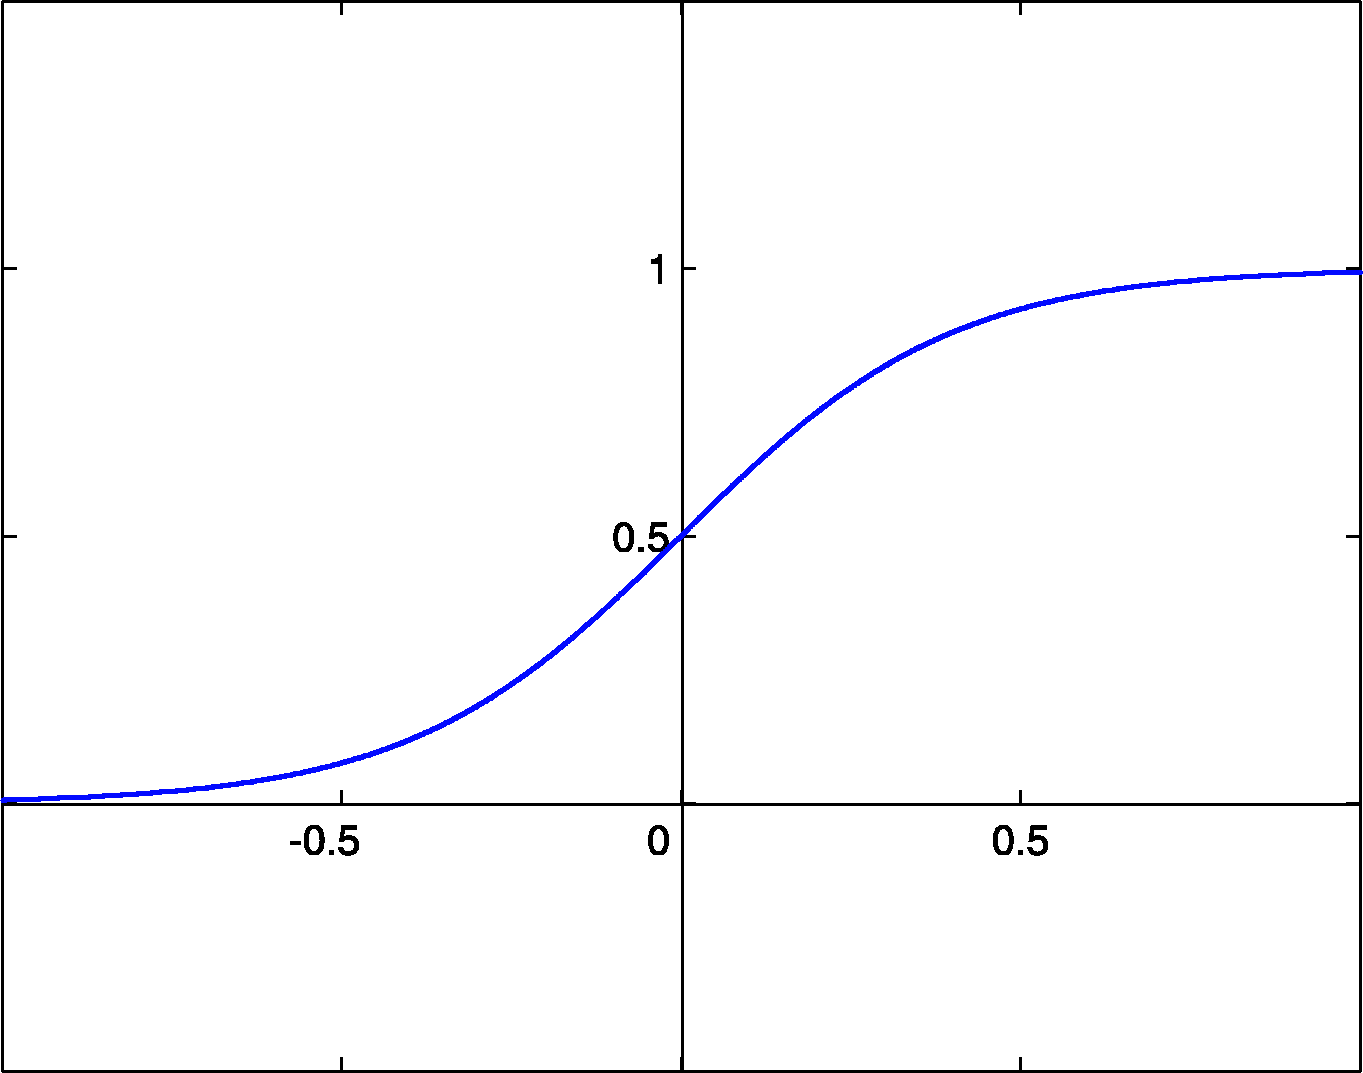
\includegraphics[width=4in]{SigmoidFunction}
  \caption[]{Log-Sigmoid Function. Credit: wikibooks.org}
  \label{SigmoidFunction}
\end{figure}

The output of the function is bounded by [0,1] and the value of the function is expressed as:

\begin{align*}
\sigma(t) = \frac{1}{1 + e^{-t}}
\end{align*}

Many of these Neurons are connected in layers where the outputs of one layer become the inputs of another layer.

\subsubsection{Feature Extraction}
In order to classify an input, features associated with the input must be extracted. These features can be pixel intensities, frequency of keywords, weights etc. This project relates to the recognition of images and the steps involved are to read the data, normalise the data, use this normalised data in the neural network. The normalisation involved is to resize the image to a fixed dimension and then apply a function to each pixel of the image bounding its intensity.
\newline
\newline
Once the images have been normalised they are passed to the first layer of Neurons, which each examine overlapping portions of the image. The reason that these portions overlap is that with images there is no guarantee that the same object will occupy the same pixels in separate images. Handwriting is inconsistent and digits may be skewed or translated relative to each other even though both images represent the same digit.

\subsubsection{MNIST Dataset}
The MNIST dataset is a collection of handwritten digits, considered the ``Hello World'' of machine learning. It consists of 60,000 training examples and 10,000 testing examples, which are all accurately labelled. This project will be using the MNIST dataset in the evaluation of a work stealing algorithm. The set of training images will be divided into distinct subsets, and workers will be assigned a subset to train on. The benefit of dividing the images is that it will be faster to process these images in parallel and aggregate results rather than inspecting each image individually.

\subsubsection{Distributed Machine Learning}

There already exist many solutions to the problem of distributed machine learning. The main difference between a single worker and multiple workers is the need to synchronise each worker's model. There are two schemes for doing so: with a centralised store that all workers communicate with, or a decentralised version where workers exchange updates to each other. The decentralised version requires $\mathcal{O}(n^2)$ messages to be exchanged as each worker must communicate with all others. But the centralised version requires only $\mathcal{O}(n)$ messages. In order for the solution to scale well, the version with the lower message complexity must be chosen. This architecture will be discussed in more detail in Section \ref{paramserver}.
\newline
\newline
An example of the centralised version is the Bosen system \cite{wei2015managed}, designed to scale to a cluster of at least 1024 cores and limits the amount of bandwidth used in its inter-worker communications to below a specified amount. However, Bosen does not consider the impact of stragglers.

\subsection{Parameter Server Architecture} \label{paramserver}
This project will investigate the effects of work stealing in a distributed machine learning framework. The advantage of a distributed framework are decreased training time, redundancy in the event of a single machine failing, and allowing training to occur on datasets that cannot fit on a single machine.
\newline
\newline
In the parameter server environment there are two processes controlling the machine learning: the parameter server, acting as a datastore of the model, and the worker, updating the model based on new training data. Data is read by the single worker and processed in batches, referred to as ``minibatches'', where a single minibatch is processed each round. Updates based on the images trained on are sent to the master at the end of each round. At the start of each round each worker receives the latest model from the master and the updates at the end of each round represent augmentations of the local model.
\newline
\newline
Figure \ref{ParameterServerArchitecture} contains a visualisation of the parameter server architecture.

\begin{figure}[H]
  \centering
  \includegraphics[width=4in]{ParameterServerArchitecture}
  \caption[]{The Parameter Server Architecture}
  \label{ParameterServerArchitecture}
\end{figure}

Algorithm \ref{SingleWorkerMachineLearningAlgorithm} is the algorithm for a single worker processing all images in rounds of minibatches. The difference in a multi-worker environment would be that the variable $i$ would only range over a subset of all possible minibatches.

\IncMargin{1em}
\begin{algorithm}[H]
 \SetKwInOut{Input}{input}\SetKwInOut{Output}{output}
 \Input{A list of all training images $N$ of size $n$}
 \Input{The size of each minibatch $m$}
 \BlankLine

$error \longleftarrow 0$\;
 \For{$i \leftarrow 0$ \KwTo $N.length/m$}{
  \For{$j \leftarrow 0$ \KwTo $m$}{
    $n \longleftarrow N[i + j]$\;
    $n' \longleftarrow normaliseImageToMatrix(n)$\;
    $prediction \longleftarrow model.train(n')$\;
    $error \longleftarrow error + computeLoss(actual, prediction)$\;
   }
 }
  $reportError(error)$\;
 \caption{Single Worker Handwriting Image Recognition Algorithm}
 \label{SingleWorkerMachineLearningAlgorithm}
\end{algorithm}
\DecMargin{1em}
\medskip

The $train()$ function processes a single data item, by feeding it forward through the Neural Network to determine the predicted output, then calculating the discrepancy between the predicted output and the actual output, and propagate this backwards through the Neural Network so that Neurons may adjust their weights to correct for errors. The $computeLoss$ function inspects the output produced by the Neural Network and determines the mean squared error between the actual output and the predicted output, equal to:

\begin{align*}
meanSquaredError = \frac{(expected - actual)^2}{2}
\end{align*}

The training of all images is known as an epoch. The errors accumulated at each worker per epoch are used to evaluate the accuracy of the system. A count is also kept of the number of correctly classified images, which is the true accuracy of the system.
\newline
\newline
In an environment with multiple workers updates to each worker's local model are sent to the master for use in synchronising workers. There are three main strategies that are used in the parameter server environment.

\subsubsection{Bulk Synchronous Parallel (BSP)}
This is the simplest form of multi-worker synchronisation. At the end of each minibatch the workers send the updates to the parameter server which collects them and will not allow workers to proceed to the next batch until all updates have been received. The advantage of this strategy is that it guarantees that all workers will converge on a single model because workers by definition cannot display more than a single round of divergence in their models. There are however significant overheads in terms of waiting for the slowest worker per round to synchronise with the master. Traffic patters are also quite bursty with the potential for network congestion at the beginning of each minibatch round. This model allows for the greatest progress in a single round because all workers operate with the latest set of parameters which provides the greatest \textit{per-data-sample} progress \cite{langford2009slow}.

\subsubsection{Full Asynchronous}
If we consider $l$ to be the limit of the number of minibatch rounds between the slowest and fastest workers then we can consider BSP to have $l = 1$. In a Fully Asynchronous model then $l = \infty$, i.e. workers proceed at their own rate unimpaired by the progress of others. Fully asynchronous models will saturate compute capacity, a metric we wish to optimise for. However, because there is no guarantee on them receiving updates from other workers before proceeding on to the next minibatch, there is the possibility that the worker's local model is stale and outdated. This reduces the efficacy of training and will result in a slowed convergence. Worker's local models may also diverge resulting in an ineffective global model at the parameter server.

\subsubsection{Bounded Staleness}
In a Bounded Staleness model $l$ is configurable. In the event of a slow worker being caused by an transient delay, for example a pathological kernel scheduling, unaffected workers can continue to make progress and the delayed worker will hopefully catch up. If a worker is consistently slower, as could be the case with a less powerful host machine, then the same problems will occur with BSP, albeit with a difference of multiple minibatch rounds, rather than one. An important result is that it is possible for workers that diverge by a fixed number of rounds to still converge on a single model \cite{NIPS2013_4894}. Without such a result, Bounded Staleness would not provide much practical use as the converge of a global model is the most important feature of a distributed machine learning environment.
\newline
\newline
In a conventional machine learning framework, the computation and updating of local parameters will be performed separately. The intention is to saturate all possible resources, which is only attainable if the separate processes are decoupled.
\newline
\newline
The algorithm for a multi-worker environment is very similar to that of a single worker as can be seen in the difference between Algorithm \ref{SingleWorkerMachineLearningAlgorithm} and Algorithm \ref{MultiWorkerMachineLearningAlgorithm}. Note that the worker no longer accepts all training images, but rather a subset of them, and that the concept of a staleness bound has been introduced to prevent divergence between the workers.

\IncMargin{1em}
\begin{algorithm}[H]
 \SetKwInOut{Input}{input}\SetKwInOut{Output}{output}
 \Input{A list of this worker's training images $N$}
 \Input{The size of each minibatch $m$}
 \Input{The limit of staleness between the slowest and fastest workers $l$}
 \BlankLine

 $round \longleftarrow 0$\;
 \For{$i \leftarrow 0$ \KwTo $N.length/m$}{
  \While{$round - l > globalRound$}{
    \tcc{Busy wait until the staleness limit has been reached}
  }
  \For{$j \leftarrow 0$ \KwTo $m$}{
    $error \longleftarrow 0$\;
    $n \longleftarrow N[j]$\;
    $n' \longleftarrow normaliseImageToMatrix(n)$\;
    $grad \longleftarrow extractGradients(n')$\;
    $prediction \longleftarrow model.train(grad)$\;
    $error \longleftarrow error + computeLoss(actual, prediction)$\;
   }
  \tcc{This will send updates to the parameter server}
  $model.correctError(error)$\;
  $round \longleftarrow round + 1$\;
 }
 \caption{Multiple Workers Handwriting Image Recognition Algorithm}
 \label{MultiWorkerMachineLearningAlgorithm}
\end{algorithm}
\DecMargin{1em}

\medskip
\medskip

Algorithm \ref{MultiWorkerMachineLearningAlgorithm} and Algorithm \ref{ModelUpdate} execute in parallel on seperate threads per worker to ensure the greatest use of resources possible.
\newline

\IncMargin{1em}
\begin{algorithm}[H]
  $globalRound \longleftarrow 0$\;
  \While{$true$}{
    $update \longleftarrow receiveParameterServerModelUpdate()$\;
    $model.applyUpdate(update)$\;
    $globalRound \longleftarrow globalRound + 1$\;
  }
 \caption{Model Update}
 \label{ModelUpdate}
\end{algorithm}
\DecMargin{1em}
\medskip

\newpage

\section{Work Stealing Algorithms} \label{algorithms}

To implement work stealing between workers in a parameter server architecture two algorithms were developed. One of which focused on a decentralised, worker-to-worker communication model, and another using the parameter server as a central co-ordinator. This chapter will discuss the implementation of both algorithms as well as considerations for real world use.

\subsection{Centralised Model}

The centralised approach is based upon workers sending periodic updates to the master with their current status. The interval between these updates is configurable, but through evaluation of these intervals I have found that diminishing returns occur beyond 5 intervals per round. With more than 8 workers, this limit drops to 3 as workers begin to overwhelm the Parameter Server with update messages.
\newline
\newline
Updates to the master occur multiple times per round for each worker, and each round is usually completed within 40-80ms per worker depending on number of cores available. The diminishing returns occur due to a linear performance profile during each round for workers. In the event of a performance degradation, the cause is unlikely to be resolved within a single round. Therefore while certain rounds contain the start of a transient event that affects performance, most rounds occur in either an optimal or degraded state, and do not alter between within a single round. This can be seen on Figure \ref{RoundDegradation} which shows how transient events affect multiple rounds. This result was achieved by inducing a CPU intensive process during machine learning training. Note the very sudden increases in time per round indicating that these events occur very quickly. The precision of the graph is not fine enough, but the raw data reveals that this increase in average time occurred within a single round.

\begin{figure}[H]
  \centering
  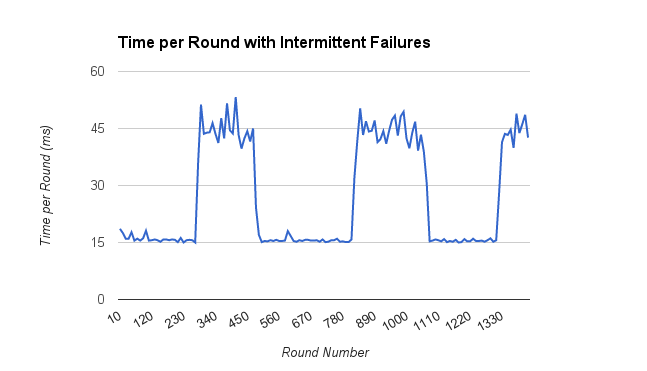
\includegraphics[width=4in]{RoundDegradation}
  \caption[]{Graph showing effects of transient events}
  \label{RoundDegradation}
\end{figure}

Updates beyond a certain frequency simply represent no new information and simply cause to increase load on the parameter server and utilise excessive bandwidth.

\subsubsection{Update Based Approach}
Initially, four centralised notification exchange schemes were considered and benchmarked to determine which provided the greatest benefit against stragglers.

\begin{enumerate}
\item No updates and message sent before end of round.
\item No updates and message sent at end of round.
\item Updates and message sent before end of round.
\item Updates and message sent at end of round.
\end{enumerate}

The distinction between \say{end of round} and \say{before end of round} refer to when the centralised master would send the messages indicating to workers how they would be affected by work stealing. Immediately the first approach can be ruled out as the master cannot know whether a worker is close to completing their round without updates. Such a system could have depended upon prior rounds and projecting round completion into the future, but this would be vulnerable to unexpected delays, which was the intention of the project.
\newline
\newline
The benefits of sending messages before the end of the round is that it allows the worker that is stealing to pre-load their image buffer so that immediately upon terminating its initial batch it could process the stolen work. There is a concern with this approach that communication delays would cause the message alerting the victim of work-stealing to not execute certain tasks to arrive after they had been processed. This will not affect the correctness of the model as all the machine learning algorithms considered in this project are iterative in that they will be exposed to all data items multiple times. The additional exposure of a small number of elements will cause a slight divergence in the model if the element had not been trained on twice, but these repeated elements represent under 0.01\% of all training elements based on empirical evaluation.

\subsubsection{Centralised Algorithm for Workers}

Algorithm \ref{CentralisedAlgorithmWorker} details the algorithm that the workers execute. The underlying framework in this project provides the mechanisms for message delivery between workers. Messages contain a string identifying the type of message, for example either an \say{update} message to the master, or a \say{begin} message to the workers.
\newline
In Algorithms \ref{CentralisedAlgorithmWorker} and \ref{CentralisedAlgorithmServer} this messaging framework will be represented using a function \say{on}. The \say{on} function takes as parameters: the message string identifier and optionally additional parameters required to process the message contents.

\IncMargin{1em}
\begin{algorithm}[H]
 \SetKwProg{Fn}{Function}{}{}
 \SetKwInOut{Input}{input}\SetKwInOut{Output}{output}
 \Input{The size of each minibatch $n$}
 \Input{The interval to send messages $interval$}
 \BlankLine
 \Fn{on("beginRound", n, interval)}{
   $stolenThisRound \longleftarrow false$\;
   $N \longleftarrow nextMiniBatch()$\;
   \For{$i \gets 1$ \KwTo $n$}{
      \If{i mod interval = 0}{
        $sendUpdateToMaster()$\;
      }
      $train(N[i])$\;
   }
   $awaitResponse()$\;
   \If{not stolenThisRound}{
     $sendResultToServer()$\;
   }
 }
 \BlankLine
 \BlankLine
 \setcounter{AlgoLine}{0}
 \BlankLine
 \Fn{on("nack")}{
 }
 \BlankLine
 \BlankLine
 \setcounter{AlgoLine}{0}
 \Input{The amount of work stolen $count$}
 \BlankLine
 \Fn{on("lose", count)}{
   $skipImages(count)$\;
 }
 \BlankLine
 \BlankLine
 \setcounter{AlgoLine}{0}
 \Input{The amount of work to steal $count$}
 \Input{The offset at which to read stolen work from $offset$}
 \BlankLine
 \Fn{on("steal", count, offset)}{
   $stolenThisRound \longleftarrow true$\;
   $N \longleftarrow readImages(count, offset)$\;
   \For{$i \gets 1$ \KwTo $count$}{
     $train(N[i])$\;
   }
   $sendResultToServer()$\;
 }
 \caption{Centralised Algorithm executed by workers}
 \label{CentralisedAlgorithmWorker}
\end{algorithm}
\DecMargin{1em}
\medskip

In Algorithm \ref{CentralisedAlgorithmWorker}, $sendUpdateToMaster()$ and $sendResultToServer()$ are simply convenience methods to communicate with the parameter server, and will not be included for clarity. The $train$ function trains the machine learning model with the specified image. $skipImages$ will skip the specified images from the end of the worker's current minibatch. A \say{steal} message will instruct the worker to read the images that another worker has been too slow to process. \say{lose} is the equivalent call to the victim of work stealing to indicate that a number of images have been lost and that they should skip them when training. \say{nack} is used to indicate that no action should be taken this round as all workers are operating at a rate similar enough that any attempt at work stealing would incur additional overhead.

In Algorithm \ref{CentralisedAlgorithmWorker} there is a call to $awaitResponse()$. This is a method which blocks execution until the worker has received either a \say{nack}, \say{lose}, or \say{steal} message and handled its body. Message delivery in this system is designed to be asynchronous, so that messages can be received and handled simultaneously. The system has also been designed so that there is a guarantee that a worker cannot receive a \say{beginRound} message until the completion of this current round. The usage of this message can be seen as an equivalent to a logical clock in that it imposes an ordering on the modification of state in the system. If a worker were to steal work it can be ensured that they would not call $sendResultToServer$ more than once per round. Figure \ref{awaitResponse} shows the necessity of such a blocking call and how the logical ordering of events is able to prevent race conditions in a way that physical clocks can not.
\newline
\newline
There exists an implicit Lamport logical clock which imposes a logical ordering between the sending of updates to the master and whether or not to immediately send a response to the master after the completion of training. It ensures that the $sendResultToServer$ event must occur after the instruction issued by the server by implicitly incrementing a Lamport logical clock only after a message from the server has been processed.
\newline
\newline
As mentioned previously, there is the potential for some images to be repeated while processing. If the server instructs a worker to skip images and the worker receives the message after beginning to process images then the will be processed twice. A variant of this algorithm which utilises a Two-Phase Commit would alleviate this problem. The server would send an initial \say{commit-request} message to workers and would receive responses indicating whether they were prepared for work stealing. The preparation would be whether the victim had not already processed the work to be stolen. Upon a successful round of responses the master would then send a \say{commit} message which would instruct the work stealing to occur. If the initial responses indicated that work stealing would not be possible this round then the master would send an \say{abort} message and no work stealing would occur.
\newline
\newline
This algorithm would achieve resiliency against the same image being processed multiple times, however the Two-Phase Commit is known for being a high overhead approach, and in this scenario the overhead outweighs the benefits.

\subsubsection{Centralised Algorithm for Parameter Server}

The algorithm which is executed by the parameter server is primarily centred around worker co-ordination and updating the central model, and is represented by Algorithm \ref{CentralisedAlgorithmServer}.

\IncMargin{1em}
\begin{algorithm}[H]
 \SetKwProg{Fn}{Function}{}{}
 \SetKwInOut{Input}{input}\SetKwInOut{Output}{output}
 \Input{The result of a worker's training $result$}
 \BlankLine
 \Fn{on("receiveResult", result)}{
   $globalModel.add(result)$\;
   $responses \longleftarrow responses + 1$\;
   \If{$responses = numberOfWorkers$}{
     $sendToWorkers("beginRound")$\;
     $responses \longleftarrow 0$\;
     $stolenThisRound \longleftarrow false$\;
   }
 }
 \BlankLine
 \BlankLine
 \setcounter{AlgoLine}{0}
 \BlankLine
 \Input{The worker sending the message $worker$}
 \Input{The latest value trained $value$}
 \BlankLine
 \Fn{on("update", worker, index)}{
   $workerProgress[worker] = index$\;
   \If{$index > stealingThreshold \land \neg stolenThisRound$}{
     $slowestWorker \longleftarrow determineSlowestWorker(workerProgress)$\;
     $workToSteal \longleftarrow calculateWorkToSteal(slowestWorker)$\;
     \uIf{$workToSteal \geq minimumStealingAmount$}{
        $send(slowestWorker, "lose", workToSteal)$\;
        $send(worker, "steal", workToSteal)$\;
        $sendTo(allWorkers - slowestWorker - worker, "nack")$\;
        $stolenThisRound \longleftarrow true$\;
     }
     \Else{
        $sendToAllWorkers("nack")$\;
     }
   }
 }
 \BlankLine
 \caption{Centralised Algorithm executed by parameter server}
 \label{CentralisedAlgorithmServer}
\end{algorithm}
\DecMargin{1em}
\medskip

Algorithm contains some convenience methods for illustrative purposes, whose contents will not be shown for brevity. The parameter server contains a variable, $responses$ which tracks the number of worker models that the server has received in a single round. $workerProgress$ is a map with keys corresponding to the identifiers of workers, and values of the latest result received from each worker.
\newline
The $send$ function is used to deliver messages to the specified worker, using the second parameter as the message identifier and all remaining parameters as message contents. $sendTo$ broadcasts a message to a specified subset of all workers, and $sendToAllWorkers$ is a simple broadcast.
\newline
$determineSlowestWorker$ traverses the mapping pairs to determine which of the workers has the lowest associated value, indicating that the worker has made the least progress this round. $calculateWorkToSteal$
is a function which will determine the amount of work to steal from the slowest worker, and this amount will then be evaluated to determine whether it will be time effective to steal work. The benefit of work stealing is that the overhead of exchanging work is outweighed by the time saved through slower workers having less work to process. If the amount of work that could be stolen this round is too low then it will be more effective to let all workers finish without the aide of work stealing.

\subsubsection{Minimum Sufficient Work Stealing Value}
The limit on the minimum amount of work that can be stolen at a benefit to the system is determined through the evaluation of the costs associated with work stealing. Initially a model will be built assuming that updates are not sent, and a simpler model will be developed once updates are added to the system.
\newline
\newline
Several per-system and per-round values are used in the generation of the model.
$t_1$ represents the time of completion of the fastest worker.
$t_2$ represents the time of completion of the slowest worker.
$r_1$ represents the rate of training for the fastest worker.
$r_2$ represents the rate of training for the slowest worker.
$l$ is the worker-parameter server message delay time.
$i$ is the time taken for the fastest worker to read the images stolen from the slowest worker.
$s$ is the time taken to send the round model from a worker to the parameter server.
$x$ is the number of images that have been stolen.
$l$ is the cost of sending a message to the server alerting that work has finished.

We can formulate these terms into the following approximation modelling the effects of work stealing.
\begin{align*}
t_1 + \frac{x}{r_1} + 2l + i + s \approx t_2 - \frac{x}{r_2} + s
\end{align*}

If updates are used then the cost of both of those messages, as well as the cost of reading the images to be stolen, will in the average case reduce to no cost. Using updates allows the server to co-ordinate workers before they have finished their initial batches, and therefore no extra overhead results. Note that the $s$ value can also be ignored, as it is constant for both the victim of work stealing, as well as the worker stealing work.
\newline
The reformulated approximation to account for updates is then.
\begin{align*}
t_1 + \frac{x}{r_1} \approx t_2 - \frac{x}{r_2}
\end{align*}
$t_2$ is not a fixed value as it will occur in the future and therefore a prediction of its value shall be used instead. At $t_1$ the slower worker has $m$ images left to process this round, and would have $m -x $ images left after work stealing. Therefore an estimate for $t_2$ is $t_1 + \frac{m-x}{r_2}$, using a linear regression based on the training rate achieved by the slower worker this round. As mentioned previously, the assumption used is that in the average case that workers maintain a constant training rate per round.
\newline
The approximation can therefore be rewritten as.
\begin{align*}
t_1 + \frac{x}{r_1} \approx t_1 + \frac{m-x}{r_2} - \frac{x}{r_2}
\end{align*}
\newline
A rearrangement of this approximation to solve for $x$ leads to.
\begin{align*}
x \approx \frac{r_1m}{r_2 + 2r_1}
\end{align*}
$m$ can also be approximated as the exact value at $t_1$ is not known. All workers begin each round with $I$ images to process, and using another linear regression on the training rate the following approximation can occur.
\begin{align*}
m \approx I - t_1r_2
\end{align*}
\newline
Which leads to a final approximation of x.
\newline
\begin{align*}
x \approx \frac{r_1(I - t_1r_2)}{r_2 + 2r_1}
\end{align*}

These values are all known by the server which allows it to make a high quality prediction for whether it would be beneficial to steal work this round. It is a deliberate choice to calculate these values on a per-round basis to provide the greatest level of dynamic work stealing, and also the overhead of such a calculation is minimal. The result of this approximation is defined as $minimumStealingAmount$ in Algorithm \ref{CentralisedAlgorithmServer}.

\subsection{Decentralised Model}
The decentralised model operates on a worker-to-worker level for arranging whether work-stealing shall occur. It uses many of the same techniques as the centralised model, but the parameter server is used solely as a store for the machine learning model.
\newline
\newline
The benefit of the system is that the logic for determining whether to steal work is co-located with the state responsible for tracking worker progress. The initial reasoning for the efficacy of the decentralised model was that it would attempt to reduce overhead by removing additional messages.

\subsubsection{Decentralised Algorithm for Workers}

Algorithm \ref{DecentralisedAlgorithmWorkerBeginRound} details how workers handle the beginning of each round. As in the centralised version workers receive a \say{beginRound} message from the server to indicate that they should commence training on the next minibatch of images.
\newline
\newline
Using the same technique as the centralised version, workers will send a message when they approach the final message in a batch, rather than waiting to complete the minibatch. This is done as a performance improvement, and Figure \ref{RoundDegradation} shows that transient events do not tend to affect workers on a per-round basis, which leads to the simplifying assumption that each round displays a constant training rate for each worker.

\IncMargin{1em}
\begin{algorithm}[H]
 \SetKwProg{Fn}{Function}{}{}
 \SetKwInOut{Input}{input}\SetKwInOut{Output}{output}
 \Input{The size of each minibatch $n$}
 \Input{The number of workers $w$}
 \Input{The number of images to be processed before sending message $threshold$}
 \BlankLine
 \Fn{on("beginRound", n, w, threshold)}{
   $sentRemaining \longleftarrow false$\;
   $receivedRemaining \longleftarrow false$\;
   $responsesOutstanding \longleftarrow w - 1$\;
   $N \longleftarrow nextMiniBatch()$\;
   \For{$i \gets 1$ \KwTo $n$}{
      \If{$i = threshold \land \neg receivedRemaining$}{
        $send("remaining")$\;
      }
      $train(N[i])$\;
   }
   \If{$\neg sentRemaining$}{
     $sendResultToServer()$\;
   }
 }
 \caption{Centralised Algorithm executed by workers}
 \label{DecentralisedAlgorithmWorkerBeginRound}
\end{algorithm}
\DecMargin{1em}
\medskip

The logic to handle a minibatch is very similar to the decentralised system. If a worker reaches the threshold required to commence the work-stealing process and it has not received messages from other workers this round it will broadcast a \say{remaining} message. This broadcast will also set an internal boolean variable \say{sentRemaining}. After training completes workers will either send their models to the server if they were not the first to attempt work stealing, otherwise they will not.
\newline
\newline
There are guarantees imposed on further steps in the algorithm which ensure that if a worker were to send a \say{remaining} message that the local model would also be sent to the server. Thus, per round, it can be seen that all workers will send their local models, ensuring liveness in the system.

\subsubsection{Minimum Sufficient Work Stealing Value}
Similar to the centralised model there exists a minimum value for which work stealing will be beneficial. If the model in which messages are exchanged prior to round completion is considered then the resulting approximation for the number of images to steal, x,  is identical.
\begin{align*}
x \approx \frac{r_1(I - t_1r_2)}{r_2 + 2r_1}
\end{align*}
Where $r_1$ and $r_2$ are the training rates of the fastest and slowest workers respectively. The slower worker, upon receiving the message will be able to determine the faster worker's rate by accounting for a slight message delay, and it will know its own rate exactly.
\newline
Using the following equations for the value of $r_1$ and $r_2$ the approximation can be further refined.
\begin{align*}
r_1 = \frac{I(1-threshold}{t_1- l}
\end{align*}

Where $l$ is the inter-worker message delay. At time $t_1$ the slower worker has received the message but between sending the message and its arrival the faster worker will have continued to process images. The value of $t_1 - l$ is sent by the faster worker as part of the message so that the slower worker can know exactly how long it took to process up to the threshold.

\begin{align*}
x = \frac{I - rem}{t_1}
\end{align*}

Where $rem$ is the number of images remaining.
\newline
Using these values, the final approximation for the decentralised algorithm is:

\begin{align*}
x \approx \dfrac{\dfrac{I(1 - threshold)rem}{t_1 - l}}{\dfrac{I - rem}{t_1} + \frac{2I(1 - threshold)}{t_1 - l}}
\end{align*}

\subsubsection{Decentralised Algorithm Work Stealing Protocol}

Algorithms \ref{DecentralisedAlgorithmWorkerRemaining} and \ref{DecentralisedAlgorithmWorkerResponse} detail the two-way protocol which facilitates the stealing of work. In Algorithm \ref{DecentralisedAlgorithmWorkerBeginRound} it can be seen in which circumstances a worker will send a \say{remaining} message, which corresponds to the initial step of the work stealing protocol.
\newline
\newline
Upon the broadcast of the \say{remaining} message, the fastest worker awaits the arrival of a response from all other workers. This is done to impose a logical ordering on work that is stolen to ensure that a new round will not begin until all work from the previous round has completed. The remaining workers can respond with two messages types, a \say{nack} to indicate that they do not have sufficient work to steal, and a \say{remainingResponse} which instructs the fastest worker to read a number of images at a certain offset.

\IncMargin{1em}
\begin{algorithm}[H]
 \SetKwProg{Fn}{Function}{}{}
 \SetKwInOut{Input}{input}\SetKwInOut{Output}{output}
 \Fn{on("remaining")}{
  \If{$receivedRemaining \lor sentRemaining$}{
    $reply("nack")$\;
  }
  $receivedRemaining \longleftarrow true$\;
  \uIf{$remainingImages > minimum$}{
    $amount \longleftarrow determineAmountToSteal(remainingImages)$\;
    $offset \longleftarrow calculateOffset(amount)$\;
    $remainingImages \longleftarrow remainingImages - amount$\;
    $skipImages(amount)$\;
    $reply("remainingResponse", amount ,offset)$\;
  }
  \Else{
    $reply("nack")$\;
  }
 }
 \caption{Handle initial outgoing message from fastest worker}
 \label{DecentralisedAlgorithmWorkerRemaining}
 \end{algorithm}
 \DecMargin{1em}
 \medskip

Similar to the centralised model, if a worker has at least a $minimum$ number of images remaining then it will respond with a \say{remainingResponse} message, and skip the images that will be stolen. If the minimum is not met, then a \say{nack} is sent to alert the faster worker that no work stealing shall occur.

\IncMargin{1em}
\begin{algorithm}[H]
 \SetKwProg{Fn}{Function}{}{}
 \SetKwInOut{Input}{input}\SetKwInOut{Output}{output}
 \Fn{on("nack")}{
   $reponsesOutstanding \longleftarrow responsesOutstanding - 1$\;
   \If{$responsesOutstanding = 0$}{
     $sendResultToServer()$\;
   }
 }
 \BlankLine
 \BlankLine
 \setcounter{AlgoLine}{0}
 \Input{The amount of work to steal $count$}
 \Input{The offset at which to read images from $offset$}
 \BlankLine
 \Fn{on("remainingResponse", count, offset)}{
   $reponsesOutstanding \longleftarrow responsesOutstanding - 1$\;
   $stolenImages \longleftarrow readImages(count, offset)$\;
   $awaitTraining()$\;
   \For{$i \gets 1$ \KwTo $count$}{
     $train(stolenImages[i])$\;
   }
   \If{$responsesOutstanding = 0$}{
     $sendResultToServer()$\;
   }
 }
 \caption{Handle possible responses from slower workers}
 \label{DecentralisedAlgorithmWorkerResponse}
\end{algorithm}
\DecMargin{1em}
\medskip

It is guaranteed that the fastest worker will send its local model to the server regardless of the responses received, through the use of the \say{responsesOutstanding} internal state tracker.
\newline
\newline
If the fastest worker has work to steal, it will read the images at the appropriate offset and augment its local model. The function $awaitTraining()$ is used as message handling occurs concurrently with all processing. This includes if multiple work stealing messages are received and the fastest worker must train on stolen work multiple times.

\subsubsection{Disadvantages of Decentralised Algorithm}
A major concern for the decentralised model is the lack of co-ordination between the slower workers. When using the centralised model, it can be ensured that only a single batch of stolen work is sent to the fastest worker as well as only one worker stealing work. This section shall contain an analysis of these problems, as well as mitigations in application.
\newline
\newline
Message transmissions incur a physical time delay. Figure \ref{messageInterleave} visualises how multiple workers could believe that they are the fastest worker. Based on the use of this work stealing algorithm in practise it is very common that at least two workers send \say{remaining} messages.

\begin{figure}[H]
  \centering
  \includegraphics[width=4in]{messageInterleave}
  \caption[]{Interleaving \say{remaining} messages}
  \label{messageInterleave}
\end{figure}

The following two rules define the decentralised work stealing protocol in the event of multiple workers considering themselves to be the fastest.

\begin{enumerate}
\item No worker shall have its work stolen more than once.
\item All work must be trained on.
\end{enumerate}

It is for this reason that Algorithm \ref{DecentralisedAlgorithmWorkerRemaining} contains the $receivedRemaining \lor sentRemaining$ statement. If a worker has already received a \say{remaining} message then it can have responded with either a \say{nack}, in which case any future messages should return \say{nack} as the number of images remaining decreases monotonically, or it will have responded with a \say{remainingResponse} in which case a \say{nack} should be returned to oblige with the first rule.
\newline
\newline
If message complexity is considered then the worst case is when all workers consider themselves to the fastest worker. With $n$ workers, and each worker anticipating $n-1$ responses, the message complexity would be $\mathcal{O}(n^2)$. This becomes the average case when all workers operate at the same rate, and thus an improvement could be made here. One consideration was to assign each worker a \say{skew} at the start of each round which would randomly vary when each worker would reach its threshold value. The work stealing equation would account for this skew and it would reduce the number of cases of multiple workers sending \say{remaining} messages, and the average case would be that only a single worker would send the \say{remaining} message. The other main problem with the decentralised model is the possibility of many workers sending \say{remainingResponse} messages to the fastest worker. A possible solution to this would be work \say{shedding} where the fastest worker is able to offload multiple work offers to workers it has received \say{nacks} from as it knows these workers have reached their threshold.

\newpage

\section{Design and Implementation}

The project developed on top of two existing bodies of work: SEEP, a distributed processing platform, and Ako, a machine learning framework built on top of SEEP. The choice was made as I had experience developing with SEEP and was comfortable working with its API, and Ako was a well-structured, easily-modifiable codebase which allowed someone with little machine learning experience to make major modifications and understand the impact of those changes. When I began work on modifying Ako to allow work stealing it functioned as both a single and multiple worker machine learning framework. All changes made were to augment the algorithms used by the workers to allow for work stealing and dynamic minibatch processing. Both of these changes will be covered in detail in this section.

\subsection{Machine Learning Framework}

Other machine learning frameworks were considered, such as Google's Tensorflow, Caffe, Theano, and deeplearning4j. Major concerns were the ability to work with a distributed system, as the basis for this project was mitigating the impact of stragglers in a multi-worker environment. This meant the exclusion of Theano, and also Tensorflow as a distributed version of the framework was not released until some time after beginning the project. Of the remaining frameworks Caffe is C++ based, while deeplearning4j and Ako are Java based. Based on personal programming experience, the choice was made to develop using Java, as I have a much greater level of experience and the language constructs for the algorithms are much simpler to use in Java. This removed Caffe as an option. Ako is a simpler framework than deeplearning4j and is designed to be less general, and as a result is less complex. While this would limit its viability in a commercial setting, as a baseline from which to develop on it was a much better choice than deeplearning4j. The modified version of Ako that has been developed also makes heavy use Java 8 Lambdas to reduce boilerplate code that adds additional visual clutter.
\newline
\newline
Note that no part of this project is dependent upon any features provided by SEEP or Ako, and that the algorithms presented would function just as well in any distributed framework.

\subsection{Dynamic Minibatch Processing}

The first feature implementation was altering how each worker processes its minibatch. This was related to the concepts presented in Section \ref{dynamicStatic}. The initial version of Ako used statically assigned work between threads and had the characteristic of resource underutilisation in the case where the amount of work to process did not divide evenly into the minibatch size. The scheduling would generate $n-1$ threads, where $n$ is the number of cores in the machine. For example, with a minibatch size of 25, and an 8 core machine, 6 of the threads would each process 3 images, and the final thread would process 7. This represented an opportunity to implement a dynamic thread scheduling. By using Java's \textit{AtomicInteger} class as the state tracker for the threads, the rate of thread processing increased significantly. Listings \ref{staticThreads} and \ref{dynamicThreads} contain an abbreviated version of the old and new scheduling code.

\begin{lstlisting}[caption={Old, static thread scheduling},label=staticThreads]
for(int i = 0; i < NUM_THREADS; i++) {
	final int IDEAL_IMAGES_PER_THREAD = (int)(examplesToTrain / NUM_THREADS);
	final int NUM_IMAGES;
	if(threadIndex < NUM_THREADS - 1) {    
    		NUM_IMAGES = IDEAL_IMAGES_PER_THREAD;
	} else {
    		NUM_IMAGES = examplesToTrain - (NUM_THREADS -1) * IDEAL_IMAGES_PER_THREAD;
	}
	for(int k = 0 ; k < NUM_IMAGES ; k++) {
		train(); // Abbreviated for brevity
	}
}
\end{lstlisting}

\begin{lstlisting}[caption={Dynamic thread scheduling replacement},label=dynamicThreads]
this.imagesRemaining.set(examplesToTrain);

for(int i = 0; i < NUM_THREADS; i++) {
    while (imagesRemaining.getAndDecrement() > 0) {
		train(); // Abbreviated for brevity
	}
}
\end{lstlisting}

The code executed inside of each of the \textit{for} loops actually is actually submitted to a Java \textit{ExecutorService} but this was omitted for brevity. When using the dynamic scheduling the average time to process each minibatch on an 8 core machine decreased from 66ms to 36ms, a ratio of 0.55 from old time to new time. Workers would execute at most 4 images now instead of 7, representing a ratio of $4/7 = 0.57$, indicating that the dynamic thread scheduling achieved almost total resource utilisation. The replacement code is also, in the author's opinion, much clearer in its intention. It is more obvious that $examplesToTrain$ items of work will be trained on, which is the contract that applies to the function.

\subsection{Normalisation}

One critical implementation design was to ensure that results were correctly normalised. Under the original version of Ako it could be assumed that at the end of each round a worker had processed one minibatch worth of images. At the end of each round workers collected the augmentations made to their local models, and would apply a normalisation step with a hard-coded value of the number of images processed. These normalised augmentations are what is sent from the worker to the global model and it is important that they represent the actual number of images trained on. Altering the normalisation logic so that a variable number of images could be used ensured that workers were correctly weighted when their updates were used by the Parameter Server. The process of tracking the amount of work actually performed by a worker in most cases is simple. Steal and Lose messages both contain the amount of work being stolen or lost, respectively. By simply adjusting for these amounts the correct value can be determined. The only possibility that this does not hold for is when a worker under the Centralised work stealing scheme processes an image before it has been instructed that the image has been stolen. In this case the amount of work lost is actually equal to the number of items remaining on receipt of the message. The number of remaining images is tracked during processing so this is a simple check of which is smaller between the number of images in the Lose message, and the actual number of images remaining.

\subsection{Architecture}
SEEP requires that computations are expressed as directed graphs where vertices represent tasks, and edges represent the ability for tasks to communicate. Ako on SEEP requires the following tasks:

\begin{enumerate}
\item Source for reading data
\item Sink for emitting the results of training
\item Parameter Server for maintaining global state
\item A variable number of Workers, each represented as its own task
\end{enumerate}

SEEP tasks are represented as Java objects which implement the \textbf{SeepTask} interface. The most important methods that must be implemented in the interface are \textbf{setUp}, used as a run-time constructor, and \textbf{processData}, used to handle incoming messages. Messages in SEEP are required to conform to a schema imposed when constructing the edges in the directed graph. Schemas in SEEP are a set of key-value pairs, with keys being strings representing the name of the value, and the value being of a fixed type. Listing \ref{AkoSchema} is the schema used in Ako for inter-task communication.

\begin{lstlisting}[caption={The SEEP schema used for Ako},label=AkoSchema]
Schema schema = Schema.SchemaBuilder.getInstance()
                .newField(Type.STRING, "task")
                .newField(Type.BYTES, "content")
                .build();
}
\end{lstlisting}

The \say{task} field is used to identify the type of message, such as: \say{beginRound}, or \say{remaining}, and content is a byte array. The rigidity of the schema imposed some issues, such as requiring to convert Java integers into a byte array representation during transmission even though SEEP does contain the ability to handle integers in a schema. However, this issue was solved using the \textbf{ByteBuffer} class in Java which allows for the serialisation of numeric types.
\newline
\newline
Figure \ref{AkoGraph} is the SEEP graph when Ako is using two workers. More workers were typically used, however the graph complexity increases quadratically with the number of workers and does not provide any more detail.

\begin{figure}[H]
  \centering
  \includegraphics[width=4in]{AkoGraph}
  \caption[]{The SEEP directed graph used by Ako with two workers}
  \label{AkoGraph}
\end{figure}

Ako initially was not able to exchange messages between workers as it was only required that workers communicate with the Parameter Server. The message stream numbering scheme used in SEEP is a little confusing at first. Upon construction of the SEEP tasks a user must explicitly write that two tasks are connected with a stream, and also provide a stream identifier. The confusing aspect is that when a task receives a message that the identifier associated with the message is the identifier that the sender has associated with the stream, not the receiver. Therefore a numbering scheme had to be developed to ensure that workers receiving messages knew the sender of the message, and also that for all message senders that each recipient had a unique stream identifier. Figure \ref{SEEPStreamIDs} shows the numbering scheme used with two Ako Workers, the same process is used for any number of workers but the graph complexity grows quickly without providing any additional insight so a smaller example is used.

\begin{figure}[H]
  \centering
  \includegraphics[width=4in]{SEEPStreamIDs}
  \caption[]{The stream numbering scheme between two Ako workers}
  \label{SEEPStreamIDs}
\end{figure}

All tasks in Ako follow the message-driven\footnote{https://en.wikipedia.org/wiki/Event-driven\_architecture} architecture and every action performed is in response to an incoming message. The architecture makes it very simple to develop distributed algorithms, which typically centre around the distribution of messages to progress the system.

\subsection{Tasks}

Each task in the Ako graph represents either a required SEEP construct, or a component of the machine learning framework. An explanation for the requirement and role of each task follows. 

\subsubsection{Source and Sink}

SEEP requires the presence of a Source task and a Sink task, which both implement the \textbf{SeepTask} interface. The Sink in Ako is not used, as all communication exists solely between the workers and parameter server during training. In other uses of SEEP it can act as a final aggregation point collecting the results of many previous tasks and collate them into a single data source. If for example a word count program were developed and the corpus of text too large to fit within a single machine then there could be many workers each processing a subset of all text and sending their results to the sink to publish the final results in a log file. The sink is only required to handle word frequencies and therefore only a single machine would be required to aggregate all results.
\newline
\newline
In Ako, the state of the parameter server can be saved to a file, and loaded during another training run so as to not commence from a completely untrained model each time. The Source is responsible for loading the saved model from a file and sending to both the workers and parameter server. As can be seen in Figure \ref{ControlFlow} which visualises the relation between the Source, Parameter Server, and Workers.

\begin{figure}[H]
  \centering
  \includegraphics[width=4in]{ControlFlow}
  \caption[]{Control Flow between components}
  \label{ControlFlow}
\end{figure}

\subsubsection{Parameter Server}

The Parameter Server is responsible for receiving and applying updates to the global model from workers, and also to co-ordinate the rounds of minibatches that will be processed. It's functionality is stored in the \textbf{ParamServer} class.
\newline
\newline
All classes in Ako use the Java Kryo library \cite{kryo} for object serialisation and all serialised objects are represented as byte arrays to conform to the SEEP schema. After the update from the worker has been de-serialised, it is used to augment the global model. Once the number of updates equals the number of workers then a round is complete, and the parameter server will send a message to alert the workers to commence a new round.
\newline
\newline
Listing \ref{ParameterServerParallel} details the Java code executed by the Parameter Server. Some method and variable names have been changed for brevity, but this is an accurate representation of the work performed by the Parameter Server.

\begin{lstlisting}[caption={Parameter Server message handling},label=ParameterServerParallel]
int sid = dataTuple.getStreamId();
byte[] bytes = dataTuple.getBytes("content");

ModelNN gradients = deserialise(sid, bytes);

//Apply gradient to the neural-net model in this param server
applyUpdate(gradients);
counter.incrementAndGet();

if (counter.compareAndSet(numReplica, 0)) {
    //Extract only the weight from the current neural-net model state
    ModelNN weightOnlyModel = ModelNN.extractWeight(getCurrentModelNNInstance());

    byte[] weightOnlyModel_bytes = serialise(sid, weightOnlyModel);

    byte[] newGlobalModel = OTuple.create(schema,
            new String[]{"task", "content"},
            new Object[]{BEGIN_ROUND, weightOnlyModel_bytes});

    for (int i : workerIDs) {
        api.sendToStreamId(i, newGlobalModel);
    }
    round++;
}
\end{lstlisting}

Line 7 is the statement for updating the global model based on updates received from workers. Once $numReplica$ messages have been received the Parameter Server knows that a round has terminated, it generates a copy of the latest global model to distribute and sends it to all workers. Messages sent are a series of unicasts as SEEP uses TCP for inter-worker communication, and TCP does not offer the ability to broadcast. A future extension may be to allow the use of alternate protocols to facilitate broadcasts.
\newline
\newline
An attempt to convert the message processing of the Parameter Server was attempted. It introduced a large mental overhead to determining how to handle the possibility of multiple threads executing Listing \ref{ParameterServerParallel} concurrently as there was the potential for many, subtle data races. An evaluation of the serial vs concurrent versions was performed, and there was no significant performance improvement when using the concurrent version. The time taken to process a single message was within 2ms and the messages received by the Parameter Server were often spaced by more than that amount apart implying that there could not have been a significant performance improvement. The code was reverted to the serial implementation and has functioned without issue across several hundred thousand rounds of evaluation.

\subsubsection{Worker}

The workers are responsible for processing of images, augmenting their local models, and after finishing a minibatch, to send them to the parameter server. The workers were initially designed to only handle one type of message per round, so a significant effort was made to convert the system into an asynchronous model. This applies to both the centralised and decentralised models, as both have message types to respond to while training.
\newline
\newline
Workers make heavy use of Java concurrency primitives to ensure thread safety and no data races. Languages such as Rust are able to remove the possibility of data races with the compiler, and this would have been an incredibly useful aide during programming as subtle bugs were common. Java contains a concurrency tool \textbf{Future} which represents the result of an asynchronous computation. It was used to ensure that a single worker would not block on the loading of images that it had stolen. The \textit{synchronized} keyword also made reasoning about control flow much easier as it guarantees that for a single instantiation of an object that a certain method cannot be called concurrently by more than one thread. An ideal use case for this was the \textbf{train()} method, where training on stolen work should be delayed until the initial training is complete, but should also execute as soon after as possible. Workers would call the the \textit{train()} method after having loaded the stolen images and execution would continue as soon as the initial training had completed. Listing \ref{AsyncImages} contains the Java code executed by the workers when reading images. The $readFromStolenBuffer$ field is used to ensure that while training that a worker reads its own images and while stealing work it only reads stolen images. The images are read before proceeding to train on the stolen work and through profiling of the Java code it was found that the image reading does not impede the progress of the Java code.

\begin{lstlisting}[caption={Image Reading},label=AsyncImages]
// Now read the stolen images to the buffer while initial training continues.
readStolenImagesToBuffer(workStolenCount, senderID);

// Block for the current batch of training to finish.
try {
    currentTraining.get();
} catch (InterruptedException | ExecutionException e) {
    e.printStackTrace();
}

this.readFromStolenBuffer = true;
\end{lstlisting}


Advice for concurrent programming is to avoid mutable and global state. If the messages being passed around contain all that is needed to execute the algorithm then there is no chance of data races. Unfortunately, in order for the message size to not have a significantly adverse affect on performance, they can only contain references and not values. Global state is also required as the messaging framework provided by SEEP is simply a method call, and Java object fields are necessary to store state between messages. The problem domain is also one that requires mutable state. The models are too large to simply create a new, immutable version on every update, and doing so would impose a heavy performance penalty for creating and garbage collecting so many objects.

\newpage

\section{Evaluation}

The primary objective of this project was to determine whether an algorithm could be developed that would mitigate the impact of stragglers in a machine learning framework. The objective metric is therefore a comparison in the rate of progress that is made when stragglers are present with and without the use of work stealing. In order for the approach to be valid, the accuracy of the machine learning model must not be negatively affected by work stealing.
\newline
\newline
There are several different parameters that can effect the efficacy of work stealing, and evaluations will vary these parameters to determine their effect.

\begin{enumerate}
\item Work stealing threshold
\item Number of workers
\item Number of stragglers
\item Minibatch size
\end{enumerate}

In order to provide consistent results, stragglers will be created by either using less powerful machines that  take longer to train per round, or by introducing a CPU-intensive workload intermittently on an equally powerful machine.

\subsection{Expected Results}
Prior to running any evaluation experiments, hypotheses will be made, and the objective results will validate or reject these hypotheses.

\begin{enumerate}
\item More workers decreases training time, but at a sub-linear rate.
\item Increased cores will improve performance per worker at a linear rate.
\item The number of stragglers will severely impact the efficacy of the algorithms.
\item A larger minibatch size will correlate well with algorithm efficacy, but will result in worse accuracy.
\item The Decentralised algorithm will scale better than the Centralised.
\end{enumerate}

I believe that more workers will improve at a sub-linear rate because of communication overheads where the master will become a source of congestion. As discussed previously, in larger machine learning frameworks the parameters are sharded over many servers. This horizontal scaling allows for the number of workers to increase beyond the capacity of a single parameter server.
\newline
\newline
The centralised algorithm should theoretically handle a greater number of stragglers than the decentralised algorithm. This is because a central point of co-ordination would allow for a more even spreading of work through a single node being able to assign stolen work to multiple workers better than those same workers could arrange by themselves.
\newline
\newline
The size of each minibatch is a compromise between accuracy and training rate. If workers were to resynchronise after each image trained then the runtime would be dominated by communications between workers. Conversely, if all workers were assigned a single minibatch then model updates would only occur after all data had been trained on. We wish for each worker to have seen as much data as possible before training on a new data item, resynchronising very infrequently reduces the amount of data a worker has seen for most items in a large minibatch.
There are overheads when using work stealing: the time spent fetching images, the time spent exchanging messages, and the potential for the centralised model to train on an image twice. Work stealing messages are proportional to the number of minibatches, so a larger minibatch size would cause less overhead taken by work stealing.
However, the absolute metric that should be evaluated is model accuracy, and increased performance is rarely a more desirable metric.
\newline
\newline
The centralised model is dependent upon the parameter server handling all messages. Reading each message causes a time delay imposed by the SEEP platform. At a greater number of workers it may result in the parameter server's main functionality being delayed while work stealing messages are handled. The number of messages received per round for the parameter server is $\mathcal{O}(nm)$, where $n$ is the number of workers, and $m$ the update interval. Conversely, in the decentralised model the number of messages received per round for the fastest worker is only $\mathcal{O}(n)$. At larger values of $n$ this difference will result in a significant increase in message volume for the parameter server.

\subsection{Machine Learning Accuracy}
An expected result was that a greater number of machines that the accuracy would be lower after a give number of epochs. This is due to the greater synchronisation delays where the rate of propagation is inversely proportional to the number of workers. Conversely, the time taken to train on a single epoch is inversely proportional to the number of workers as fewer images per worker must be processed by each worker. The data collected on epoch duration was not collected in any of the experiments as it was not related to the objective of this project.
\newline
\newline
Unless specified otherwise, workers trained with minibatch sizes of 25. The larger the size of the minibatch, the longer between worker synchronisations, which leads to a worsened accuracy. 25 was chosen as it provided a good compromise between: amount of work stolen, accuracy, and message volume. An evaluation of differing sizes of minibatch is provided later.
\newline
\newline
All workers began training with a model saved from a previous training session. This offers no performance benefits against starting from a completely untrained model, but allowed insight into how workers performed at the later stages of training where differing levels of accuracy would severely impact the result of testing.
\newline
\newline
All experiments were analysed over 10 epochs of training. This limit was placed so that all workers would be compared after having seen the exact same amount of training data. This also ensured sufficient data points to allow for accurate measurements to be performed. In the worst case of 8 workers with 100 images per minibatch, there would be $60000/(8*100) = 75$ rounds per epoch, and with 10 epochs this would provide 750 data points.
\newline
\newline
The MNIST dataset contains 60,000 training images and labels, and 10,000 testing images and labels. Accuracy was measured by counting the number of correctly classified images in the testing dataset as a percentage of all images.
\newline
\newline
It was found that there was no impact on accuracy at all when using work stealing. Graphical evidence of this was found to be gratuitous and therefore it is presented as a series of tables in Appendix A. 

\subsection{Testing Environment}
All experiments were run on Amazon Web Services (AWS), a public cloud computing environment offered by Amazon.com. AWS allows customers to rent virtual servers at a range of price and performance levels. In this evaluation, all virtual servers were co-located within the same data centre, with a round-trip time of below a millisecond when using the \textit{ping} utility. There were two levels of workers, \say{healthy} workers with 16 cores of compute, and \say{stragglers}, a weaker class of server with only 4 cores of compute. The motivation for using two classes of compute was to provide a fair level of comparison between experiments. It is unlikely in industrial use for two types of machine which differ so greatly in performance to be used in the same machine learning environment. In order to provide a fair comparison between two different experiments though, it was necessary to control for straggler performance, an infamously non-deterministic factor. An evaluation with intermittent stragglers will be discussed in a later section.

\subsection{Number of workers}
The first set of experiments ran was to evaluate the impact of varying numbers of workers, and the impact of work stealing at different scales. The experiments varied over 2, 4, and 8 workers with at most a single straggler. The fastest time per round, slowest time per round, and best accuracy amongst all workers were measured. No work stealing, the centralised work stealing algorithm, and the decentralised work stealing algorithm were all compared.
\newline
\newline

\begin{figure}[H]
  \centering
  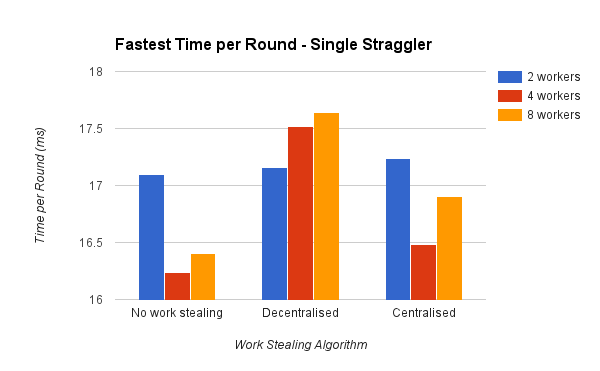
\includegraphics[width=6in]{FastestSingle}
  \caption[]{Fastest Time per Round - Single Straggler}
  \label{FastestSingle}
\end{figure}

Figure \ref{FastestSingle} shows the fastest time per round against the number of workers and work stealing algorithm used. The range between fastest and slowest measurements varies by 1.5ms. In the experiments I found that the centralised algorithm tended to be less balanced amongst workers, whereas the decentralised version spread the work stealing well across workers. This would explain why the fastest workers in the centralised version were faster than those in the decentralised, as they would routinely not steal work and thus wouldn't have the round times affected.

\begin{figure}[H]
  \centering
  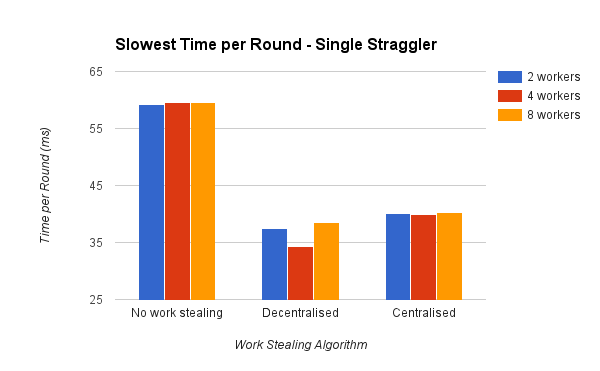
\includegraphics[width=6in]{SlowestSingle}
  \caption[]{Slowest Time per Round - Single Straggler}
  \label{SlowestSingle}
\end{figure}

Figure \ref{SlowestSingle} shows the impact of work stealing. The slowest time per round is the limiting factor regarding training rate. By stealing work, the straggler has less to do, and therefore will complete sooner. It can be seen that the decentralised algorithm was able to provide the fastest times for the slowest worker, indicating that it was the most effective algorithm. The drop at 4 workers for the decentralised algorithm was not anticipated and likely was the result of improved networking conditions at the time of evaluation.
\newline
\newline
\newline
The most important metric to evaluate was model accuracy. If this was impacted by work stealing, then the costs would outweigh the benefits. Figure \ref{AccuracySingle} shows the average accuracy across all workers after 10 epochs. It can be seen that work stealing provides a slight improvement. This was an unexpected result, and after further evaluation of the averages it was found that the workers that had stolen work had higher accuracies than when they did not steal work. This can be attributed to accuracy being a function of images read, and that with work stealing, more images were read than. The slowest worker conversely had a lower accuracy, but this was outweighed by the improvements to the faster workers.

\begin{figure}[H]
  \centering
  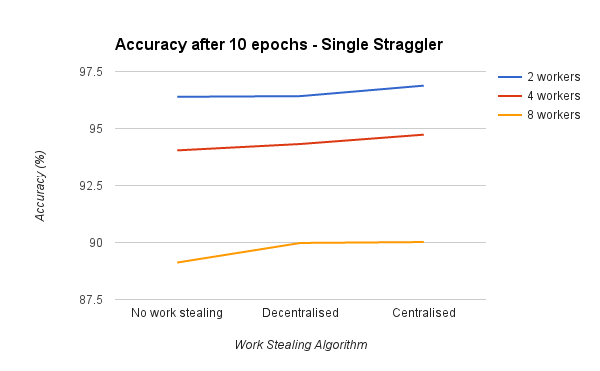
\includegraphics[width=6in]{AccuracySingle}
  \caption[]{Average Accuracy after 10 epochs - Single Straggler}
  \label{AccuracySingle}
\end{figure}

It should be noted that the improvements to accuracy were at most 0.90\%. In a subsequent experiment where the accuracy was measured after 60 epochs, it was found that the difference in accuracy would reduce to a negligible amount of below 0.10\%.

\subsection{Work Stealing Threshold}
The centralised and decentralised algorithms both use an equation to determine the ideal number of images to steal based on: rate of fastest worker, rate of slowest worker and network delays. The result of this equation is then compared to a threshold to determine if work stealing should occur. The motivation of this threshold was to prevent many small work stealings, as it was perceived that stealing a single image would result in a net decrease to training rate.
\newline
\newline
Both work stealing algorithms were run to 10 epochs with thresholds ranging from 0.0 to 0.5 with an interval of 0.1 as a proportion of the size of each minibatch. An upper limit of 0.5 was used as it can be seen in the data that the majority of work to steal was smaller than 0.5 times the minibatch size. By not stealing this work, the algorithms were less effective, and came close to the performance levels of no work stealing.

\begin{figure}[H]
  \centering
  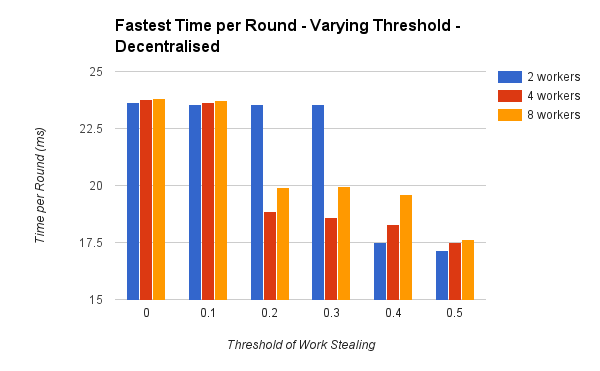
\includegraphics[width=6in]{FastestThresholdDecentralised}
  \caption[]{Average Accuracy after 10 epochs - Single Straggler}
  \label{FastestThresholdDecentralised}
\end{figure}

Figure \ref{FastestThresholdDecentralised} shows that most of the images stolen when 4 and 8 workers are used are smaller than 20\% of the minibatch size, whereas for 2 workers most are smaller than 0.40\%. This discrepancy was found to be caused by message processing overhead. With only two workers each worker is able to respond to messages more quickly as there are fewer to process per round. This means that by the time a worker sends a \say{remaining} message they will have fewer images processed, and thus can lose more.
\newline
\newline
If a worker has reached the threshold of work to send a \say{remaining} message and another worker has not completed a single image, the equation to determine the amount of work to steal will give at most half the size of the minibatch to the faster worker. This explains why at threshold = 0.5 the results are similar to those when no work stealing occurs. An improvement to the equation would be to handle this case better and ensure that the faster worker receives more than half, however this case was not encountered during training.

\begin{figure}[H]
  \centering
  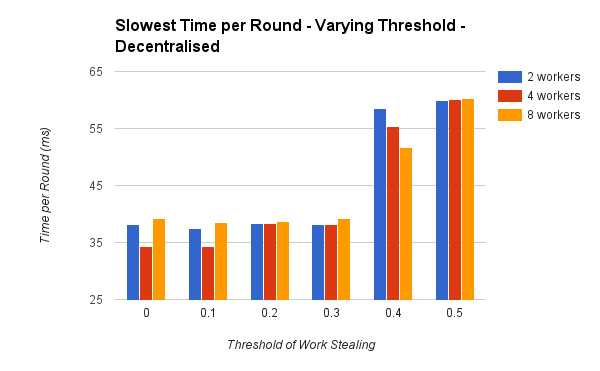
\includegraphics[width=6in]{SlowestThresholdDecentralised}
  \caption[]{Average Accuracy after 10 epochs - Single Straggler}
  \label{SlowestThresholdDecentralised}
\end{figure}

Figure \ref{SlowestThresholdDecentralised} shows slightly different results than Figure \ref{FastestThresholdDecentralised}. It appears that the slowest worker is only affected when threshold = 0.4 for worker counts. However, it was seen above that with 4 and 8 workers the significant threshold value was 0.2. The most probable cause was that there was some work stealing amongst the faster workers, although of much smaller amounts than with the straggler. By increasing the threshold to above these values the faster workers would not steal work amongst each other, only with the straggler. Note that progress is determined by the slowest worker and even with stealing amongst the faster workers the slower worker was not impacted.

\begin{figure}[H]
  \centering
  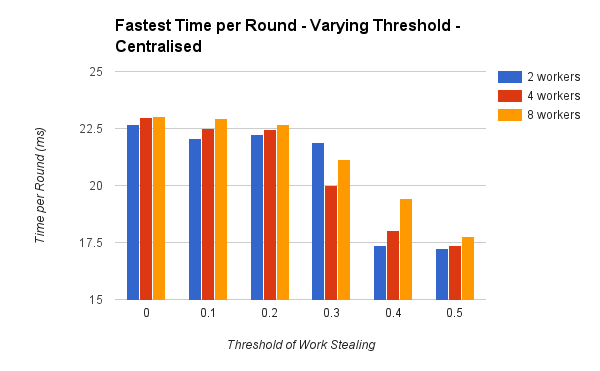
\includegraphics[width=6in]{FastestThresholdCentralised}
  \caption[]{Average Accuracy after 10 epochs - Single Straggler}
  \label{FastestThresholdCentralised}
\end{figure}

Figure \ref{FastestThresholdCentralised} confirms the evaluation of the results in Figure  \ref{SlowestThresholdDecentralised}. The centralised master prevents the healthy workers from work stealing from each other, and therefore the size of the work stolen will only be that of the straggling worker, at around 40\% of the minibatch size. The dropoff seen with the threshold at 0.3 is most prominent with higher worker counts. This is likely due to the parameter server being saturated with messages and causing delays to the work stealing messages.

\begin{figure}[H]
  \centering
  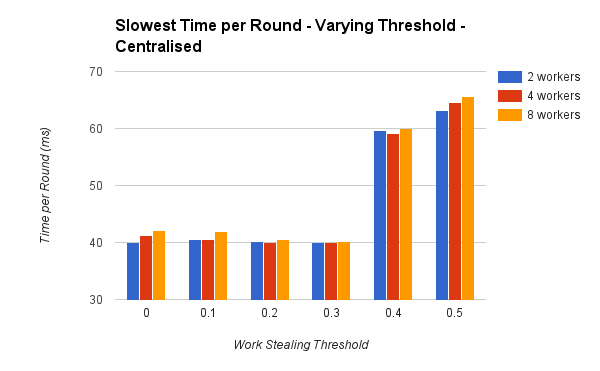
\includegraphics[width=6in]{SlowestThresholdCentralised}
  \caption[]{Average Accuracy after 10 epochs - Single Straggler}
  \label{SlowestThresholdCentralised}
\end{figure}

Figure \ref{SlowestThresholdCentralised} shows a very similar profile to the decentralised equivalent, confirming that the majority of work stolen from the straggler is smaller than 40\% of the minibatch size.

\subsection{Number of stragglers}

\begin{figure}[H]
  \centering
  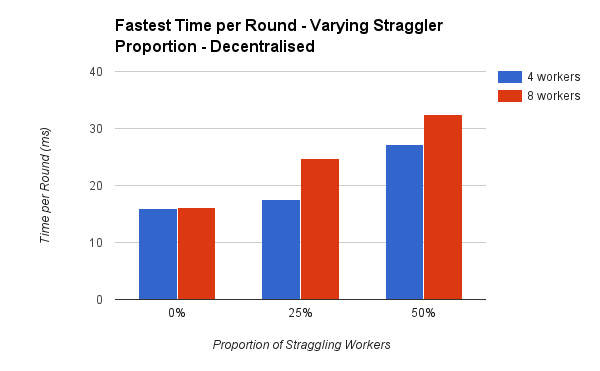
\includegraphics[width=6in]{FastestStragglerDecentralised}
  \caption[]{Average Accuracy after 10 epochs - Single Straggler}
  \label{FastestStragglerDecentralised}
\end{figure}

Increasing the proportion of straggling workers should increase the time of the fastest worker per round. This increase was due to each worker likely stealing many items of work. The impact of adding a second straggler can be seen clearly in the case with 4 workers, where there is a significant increase in the fastest worker's time per round. Two stragglers leaves results in the fastest worker having to complete two batches of work, significantly increasing its time per round. The fastest worker would alternate between the two healthy workers, and their average time per round would be therefore greater.
\newline
\newline
The increase in 8 workers was greater than anticipated. It was likely caused to communications overhead when deciding which workers to steal from. The fastest worker receives $\mathcal{O}(n)$ messages from the remaining $n$ workers which will add additional overhead.

\begin{figure}[H]
  \centering
  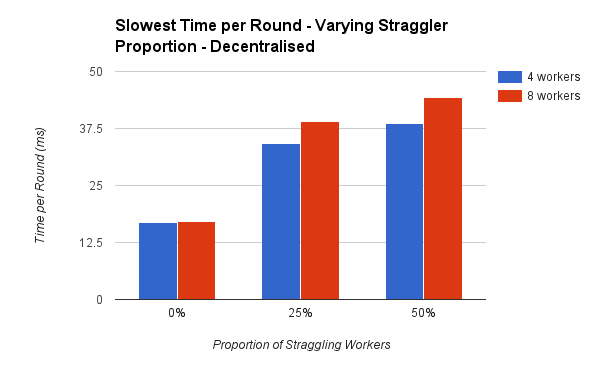
\includegraphics[width=6in]{SlowestStragglerDecentralised}
  \caption[]{Average Accuracy after 10 epochs - Single Straggler}
  \label{SlowestStragglerDecentralised}
\end{figure}

An expected result in that the slowest worker would see a drastic increase between the presence and absence of stragglers. The increase from 25\% to 50\% was small but unanticipated.

\begin{figure}[H]
  \centering
  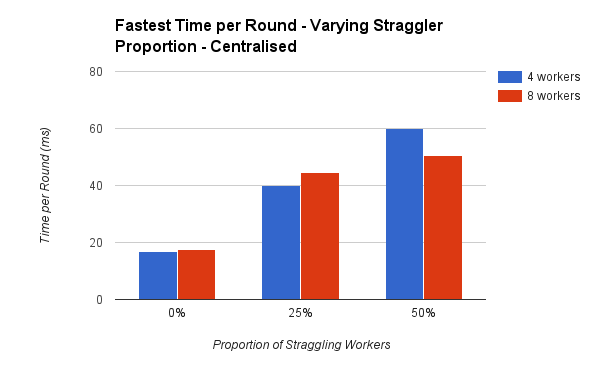
\includegraphics[width=6in]{FastestStragglerCentralised}
  \caption[]{Average Accuracy after 10 epochs - Single Straggler}
  \label{FastestStragglerCentralised}
\end{figure}

Figure \ref{FastestStragglerCentralised} results were not in line with expectations. The centralised version ensures that only one work stealing occurs per round. An assumption was that over time that the probability that any worker would be the work stealing worker would be $1/n$ with $n$ healthy workers. Since each worker was to steal only a single batch of work with a larger number of healthy workers each should have spent fewer rounds being the work stealing worker, and thus the cost of work stealing would be more greatly amortised. However, with 25\% stragglers 4 workers had a lower fastest time than 8 workers.

\begin{figure}[H]
  \centering
  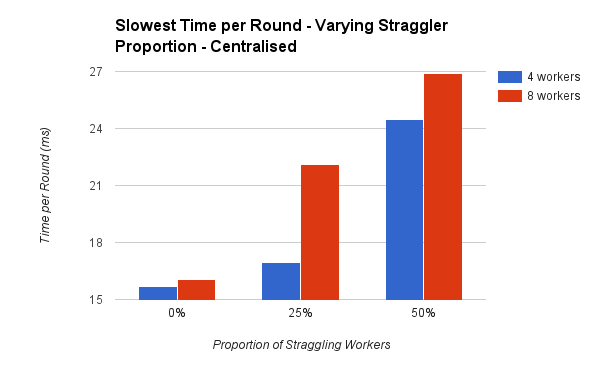
\includegraphics[width=6in]{SlowestStragglerCentralised}
  \caption[]{Average Accuracy after 10 epochs - Single Straggler}
  \label{SlowestStragglerCentralised}
\end{figure}

It is useful to compare Figure \ref{SlowestStragglerCentralised} against its decentralised equivalent, Figure \ref{SlowestStragglerDecentralised}. It can be seen that the fastest time per round is lower than the decentralised equivalent. This is evidence that the work stealing is less evenly spread, and when combined with less work being stolen per round it results in a greater difference between the fastest worker and the slowest worker. This result implies that the centralised work stealing model is less effective than the decentralised.

\subsection{Minibatch size} \label{size}

When attempting to compare minibatch size as a parameter, the aim was to show that the impact of work stealing is greater when larger minibatch sizes are used. Note that there is no value for 8 workers with a minibatch size of 10 for either of the algorithms. SEEP uses a single buffer to store messages that will be sent over a connection, and if a message is written to the buffer before another has been sent then SEEP will terminate. SEEP offers the ability to control the number of threads reading from and writing to the network, and in most of the other experiments setting 32 threads was sufficient, in this situation it wasn't. Even after setting to 128 threads the issues were not resolved. SEEP uses TCP connections, and perhaps with a lower overhead connection such as RDMA the time taken to drain the buffer to the network would be reduced and therefore no collisions would occur.
\newline
\newline
When comparing the time per round for the fastest worker it can be seen that both forms of work stealing increase the value, indicating that work stealing is occurring. However, the increase caused by the centralised algorithm is smaller than that of the decentralised, in line with expectations that the centralised version is less effective.

\begin{figure}[H]
  \centering
  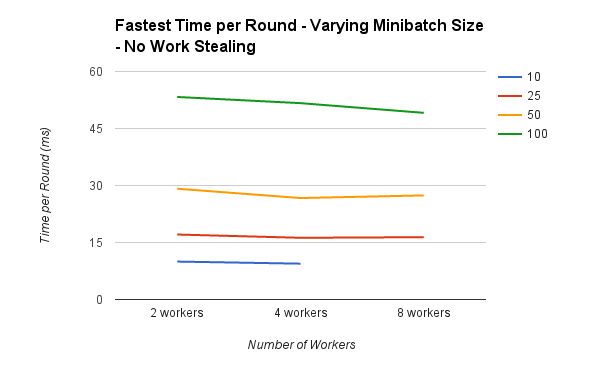
\includegraphics[width=6in]{FastestMinibatchNo}
  \caption[]{Average Accuracy after 10 epochs - Single Straggler}
  \label{FastestMinibatchNo}
\end{figure}

\begin{figure}[H]
  \centering
  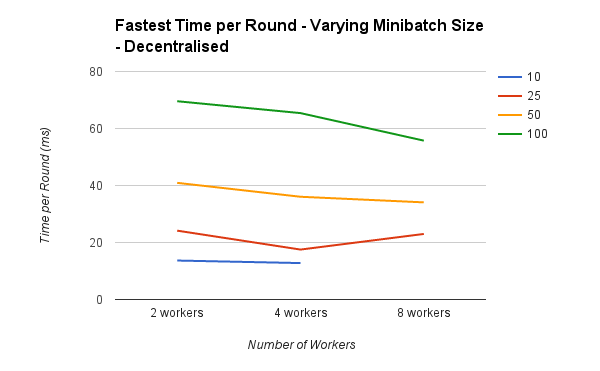
\includegraphics[width=6in]{FastestMinibatchDecentralised}
  \caption[]{Average Accuracy after 10 epochs - Single Straggler}
  \label{FastestMinibatchDecentralised}
\end{figure}

\begin{figure}[H]
  \centering
  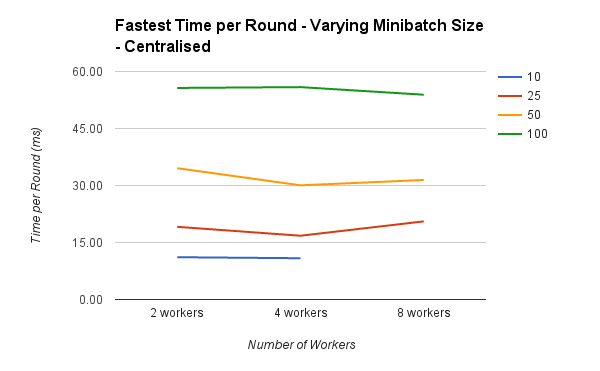
\includegraphics[width=6in]{FastestMinibatchCentralised}
  \caption[]{Average Accuracy after 10 epochs - Single Straggler}
  \label{FastestMinibatchCentralised}
\end{figure}

When comparing the run times of the straggler a confirmation of the results for the fastest worker can also be seen. The decentralised version decreases the run time of the slowest worker more than the centralised algorithm does. The difference between the two algorithms varies from 11\% at with 10 images per round, and 25\% with 100 images per round.

\begin{figure}[H]
  \centering
  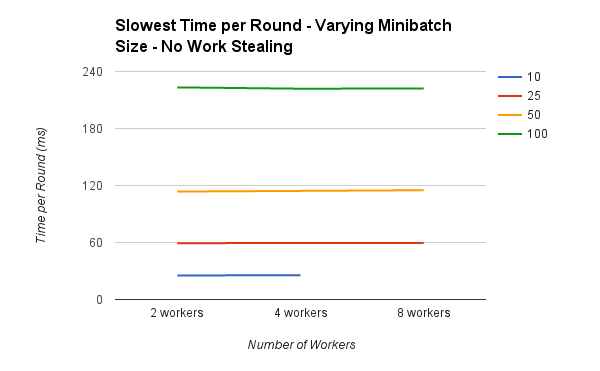
\includegraphics[width=6in]{SlowestMinibatchNo}
  \caption[]{Average Accuracy after 10 epochs - Single Straggler}
  \label{SlowestMinibatchNo}
\end{figure}

\begin{figure}[H]
  \centering
  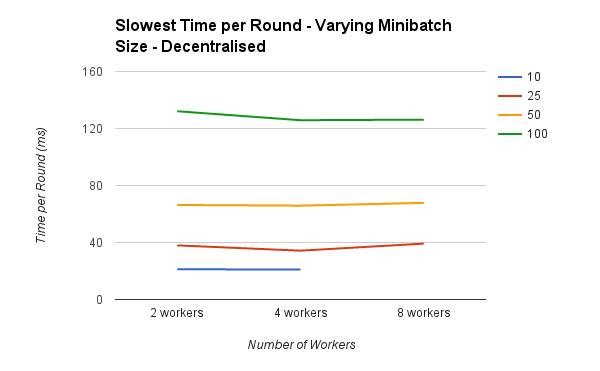
\includegraphics[width=6in]{SlowestMinibatchDecentralised}
  \caption[]{Average Accuracy after 10 epochs - Single Straggler}
  \label{SlowestMinibatchDecentralised}
\end{figure}

\begin{figure}[H]
  \centering
  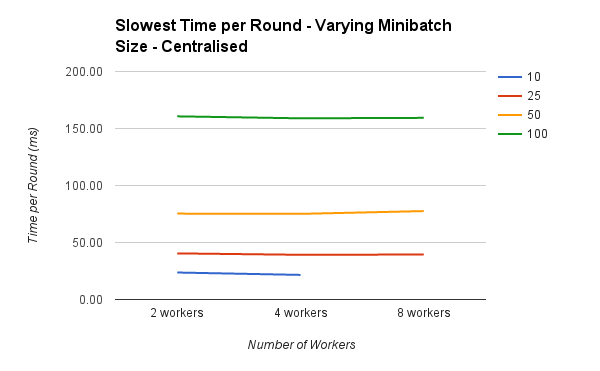
\includegraphics[width=6in]{SlowestMinibatchCentralised}
  \caption[]{Average Accuracy after 10 epochs - Single Straggler}
  \label{SlowestMinibatchCentralised}
\end{figure}

\subsection{Intermittent Work Stealing}

The above examples have all used a single straggler of a lower compute capacity than the remainder of all workers. This is unlike most machine learning environments which consist of a homogeneous collection of machines. The algorithms presented for work stealing are stateless between rounds, meaning that they should improve performance regardless of whether has been degraded for a single round, or for a prolonged period.
\newline
\newline
To evaluate this an alternate environment was used with all workers having equal performance. Training used 8 workers and a minibatch size of 25, the work stealing algorithm used a threshold of 0 images. The aim was to replicate a typical production environment used and to show that work stealing was an effective solution to intermittent load. A single worker was chosen to represent an intermittent straggler. The \textit{stress} command utility was used. It allows for a compute intensive task to be run with a variable intensity. For the 16 core machine, the task was set to saturate 8 cores thus rendering them unavailable to the machine learning framework and decreasing the worker's training rate. The comparison was performed with no work stealing and the decentralised work stealing algorithm across 1420 rounds, and the average run duration over intervals of 10 rounds was measured.

 \begin{figure}[H]
  \centering
  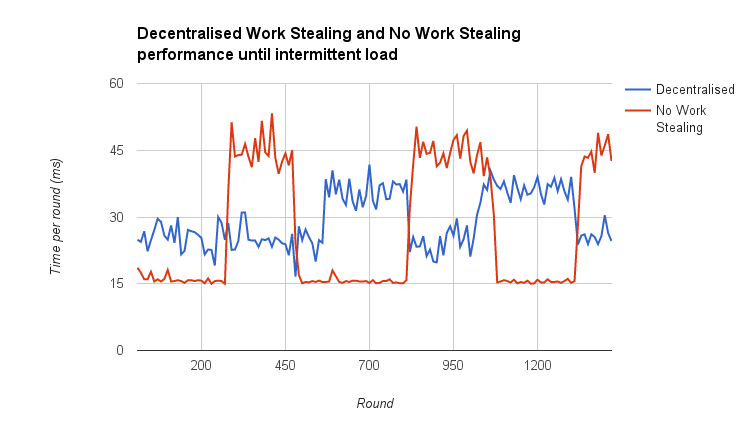
\includegraphics[width=6in]{DecentralisedVsNo}
  \caption[]{Average Accuracy after 10 epochs - Single Straggler}
  \label{DecentralisedVsNo}
\end{figure}

Figure \ref{DecentralisedVsNo} shows the impact of work stealing. Note that the \textit{stress} utility was called intermittently which is why the peaks do not align. The clear result is that even with an degraded compute performance the work stealing algorithm allowed the straggler to complete each round within a smaller amount of time. As the system is bounded by the slowest worker, this shows that work stealing aides in mitigating the impact of stragglers on the overall training rate.
\newline
\newline
The reason for the higher \say{average} round completion time for the straggler is that it was stealing work from other workers. This is a point that will be discussed in the Future Work section.

\newpage

\section{Conclusions and Future Work}

At a high level of evaluation the project was a success in that the work stealing algorithms were able to mitigate the effect of stragglers. The two algorithms presented were able to mitigate one of the most common occurrences in any large-scale system, a distribution of task durations. The algorithms also did not impair the accuracy of the trained models, which was the most important objective. The use of normalisation allowed workers to process different amounts of data without affecting the global model accuracy. An evaluation on the MNIST dataset demonstrates that the solution can be applied to industrial models. 
\newline
\newline
The variation in average run times between the fastest and slowest workers even when using the algorithms is evidence that there is still room for improvement. With a better modelling of the costs associated with work stealing it may be possible to reduce this variation to a negligible amount, a value which represents the best possible training rate achievable in such a scenario.
\newline
\newline
As discussed in Section \ref{paramserver} there are different synchronisation schemes in a machine learning environment. This project has focussed on the most-heavily restricted, Bulk Synchronous Parallel (BSP) where workers cannot diverge by more than a single round. In order to mitigate the effects of stragglers, alternate schemes such as Bounded Staleness, in which workers may diverge by more than a single round, have been used. If work stealing is able to function under the restrictions of BSP then it is also able to function under Bounded Staleness, and in fact would perform better as the size of each work stealing would be at least the size of those possible under BSP. Furthermore, if work stealing could be improved to the point of aligning the round completion times of all workers, then the need for Bounded Staleness could be removed. Due to the more frequent synchronisations between workers under BSP, it has a higher accuracy after a given number of rounds, the tradeoff being that the time per round is greater than that of Bounded Staleness. But with work stealing this would no longer be true, and thus a greater accuracy could be achieved in less time.

\subsection{Extensions}

There are several possible extensions for the project, the majority of which focus on improving performance, and the ability to scale to larger numbers of nodes.
\newline
\newline
\textbf{Optimal Work Stealing Equation}		The current equation used to determine the amount of work to steal offers a significant performance improvement over no work stolen. However, the discrepancy between the fastest and slowest workers is evidence that there is room for improvement. A more accurate model which could account for the irregular traffic patters caused by the bursty nature of the communications would allow for a reduction in the variation between fastest and slowest worker.
\newline
\newline
\textbf{Evaluation in a more controlled environment}		All of the experiments ran used Amazon's public cloud offering. This represents a typical environment used in machine learning in industry, however to achieve optimal performance it would have been beneficial to evaluate the algorithms within an environment with fewer variables. Amazon's servers are virtual servers running on physical hardware, which imposes a compute penalty. There is also no guarantee that workers are placed as physically close to each other as possible, an important concern in networking performance. It would have also been useful to evaluate in an environment with advanced technologies such as RDMA could have been used in place of unoptimised protocols such as TCP.
\newline
\newline
\textbf{Skew between workers}	One concern with the decentralised algorithm is that in the event that many workers were to reach the message sending limit at the same time that there would be many additional messages, which did not need to be sent, exchanged between workers. This did not prove to be too much of a concern in the average case, but it was an possibility that could be mitigated. Each worker would have its own local skew, computed randomly in each round, which would allow the work stealing limit to range between workers. When sending the \say{remaining} message, workers would include the skew, which would be used in the work stealing equation, and through the random value the likelihood that two workers operating at the same rate would send each other \say{remaining} messages would decrease.
\newline
\newline
\textbf{Bounded Staleness}		Although one of the conclusions of the project was that the need for Bounded Staleness may be removed when using work stealing, it would have been a useful evaluation to compare the performance of the work stealing algorithms with both Bulk Synchronous Parallel and Bounded Staleness synchronisation schemes.	
\newline
\newline
\textbf{Evaluation on Alternate Datasets}		All of the analysis was performed on the MNIST training dataset, a very widely used benchmark. It would have been interesting to evaluate the algorithms under a range of datasets. No part of any algorithm is specific to MNIST and performance under different workloads would have been interesting to analyse.

\newpage

\bibliographystyle{plain}
\bibliography{James-DavidCarr-MastersReport}

\newpage

\appendix
\section{Accuracy Results} \label{accuracyResults}

It was found that work stealing had no negative impact on the accuracy of the machine learning training. This was an important result as it was more important that accuracy be maintained than performance improved with work stealing. Appendix \ref{accuracyResults} contains the collection of recorded accuracy results after 10 epochs of training under all testing environments. All training values are the average amongst the workers present in each environment. The missing values in Tables 7, 8, and 9 are explained in Section \ref{size}.

\begin{table}[htb]
\centering
\caption{No Work Stealing}
\begin{tabular}{l | c | r}
2 workers & 4 workers & 8 workers \\ \hline
96.39     & 94.04     & 89.12
\end{tabular}
\end{table}

\begin{table}[htb]
\centering
\caption{Decentralised Algorithm - Varying Work Stealing Threshold}
\begin{tabular}{l | c | c | r}
Threshold & 2 workers & 4 workers & 8 workers \\ \hline
0                 & 96.34     & 94.18     & 89.56     \\ \hline
0.1               & 96.43     & 94.14     & 89.98     \\ \hline
0.2               & 96.42     & 94.32     & 89.41     \\ \hline
0.3               & 96.21     & 94.28     & 89.27     \\ \hline
0.4               & 96.34     & 94.08     & 89.06     \\ \hline
0.5               & 96.38     & 94.05     & 89.12
\end{tabular}
\end{table}

\begin{table}[htb]
\centering
\caption{Centralised Algorithm - Varying Work Stealing Threshold}
\begin{tabular}{l | c | c | r}
Threshold & 2 workers & 4 workers & 8 workers \\ \hline
0                 & 96.88     & 94.2      & 89.96     \\ \hline
0.1               & 96.47     & 94.33     & 89.56     \\ \hline
0.2               & 96.53     & 94.57     & 89.43     \\ \hline
0.3               & 96.51     & 94.12     & 89.22     \\ \hline
0.4               & 96.49     & 94.66     & 90.02     \\ \hline
0.5               & 96.41     & 94.73     & 89.18
\end{tabular}
\end{table}

\begin{table}[htb]
\centering
\caption{No Work Stealing - Varying Number of Straggling Workers}
\begin{tabular}{l | c | r}
\% Stragglers & 4 workers & 8 workers \\ \hline
0\%               & 94.05     & 89.26     \\ \hline
25\%             & 94.04     & 89.57     \\ \hline
50\%             & 94.05     & 89.34
\end{tabular}
\end{table}

\begin{table}[htb]
\centering
\caption{Decentralised Algorithm - Varying Number of Straggling Workers}
\begin{tabular}{l | c | r}
\% Stragglers & 4 workers & 8 workers \\ \hline
0\%               & 94.22     & 90.12     \\ \hline
25\%              & 94.32     & 90.45     \\ \hline
50\%              & 94.11     & 90.28
\end{tabular}
\end{table}

\begin{table}[htb]
\centering
\caption{Centralised Algorithm - Varying Number of Straggling Workers}
\begin{tabular}{l | c | r}
\% Stragglers & 4 workers & 8 workers \\ \hline
0\%               & 94.12     & 90.04     \\ \hline
25\%              & 94.73     & 90.13     \\ \hline
50\%              & 93.9      & 90.65
\end{tabular}
\end{table}

\begin{table}[htb]
\centering
\caption{No Work Stealing - Varying Minibatch Size}
\begin{tabular}{l | c | c | r}
Size & 2 workers & 4 workers & 8 workers \\ \hline
10                & 98.3      & 96.62     &           \\ \hline
25                & 96.39     & 94.04     & 89.12     \\ \hline
50                & 94.03     & 90.64     & 84.84     \\ \hline
100               & 90.54     & 85.25     & 80.39
\end{tabular}
\end{table}

\begin{table}[htb]
\centering
\caption{Decentralised Algorithm - Varying Minibatch Size}
\begin{tabular}{l | c | c | r}
Size & 2 workers & 4 workers & 8 workers \\ \hline
10                & 98.24     & 97.06     &           \\ \hline
25                & 96.47     & 94.18     & 89.56     \\ \hline
50                & 93.78     & 90.73     & 84.68     \\ \hline
100               & 90.71     & 84.97     & 78.77
\end{tabular}
\end{table}

\begin{table}[htb]
\centering
\caption{Centralised Algorithm - Varying Minibatch Size}
\begin{tabular}{l | c | c | r}
Size & 2 workers & 4 workers & 8 workers \\ \hline
10                & 98.33     & 96.78     &           \\ \hline
25                & 96.24     & 94.48     & 89.45     \\ \hline
50                & 93.87     & 91.03     & 84.55     \\ \hline
100               & 90.23     & 85.67     & 79.66
\end{tabular}
\end{table}

\end{document}










































